


%%%%%%%%%%%%%%%%%%%%%%%%%%%%%%%%%%%%%%%%%%%%
%%%%%%%%%%%%%%%%%%%%%%%%%%%%%%%%%%%%%%%%%%%%

\chapter{Theme 2: Closed-loop Model Checking for Implantable Pacemaker}
\label{ModelChecking}
%There are two categories of device bugs: 
%1) the device may fail to conform to its \emph{specifications}, that is, the prescription of how it should react to certain inputs.  
%2) the device may fail to improve the conditions of the patient as promised, even if it conforms to its specifications. 
%The desired physiological conditions that the closed-loop system should achieve are captured in the \emph{physiological requirements}; for example, for a pacemaker, the heart rate should always be maintained above a certain threshold. 
%
%Bugs in the first category (non-conformance to specification) can be detected via systematic and extensive open-loop testing in which a set of input sequences is fed to the device, and its output is compared with the expected output.
%Bugs in the second category (violation of physiological requirements), on the other hand, require the interaction within the \emph{closed-loop system}, which consists of the device and its environment.
%For instance, the pacemaker and the heart as its environment. 
%In the medical device industry, closed-loop verification of the physiological requirements is mostly performed in terms of clinical trials, in which the actual devices are implanted in human subjects over an extended duration.
%Unfortunately, because of the extremely high cost of clinical trials (several million dollars and spanning several years,~\cite{trialcost}), the amount and variety of human subjects during the clinical trials are limited, which reduces the opportunity to find bugs. 
%Moreover, clinical trials are often conducted at the final design stage. Fixing bugs at this stage is very costly.

Model checking is a technique in which the state space of the model under investigation is automatically and exhaustively explored to identify executions or states that violate specified properties. 
Violations of the properties are returned by the model checkers as \emph{counter-examples}, which can be used by designers to revise the design. 
In this chapter, model checking is used to evaluate an early design of a dual chamber pacemaker. 
More specifically, model checking is used to identify known and unknown physiological hazards induced by implantable pacemakers (e.g. when the pacemaker provides inappropriate therapy which drives the heart to an unsafe state).  

The chapter is organized as follow: first the basis for timed-automata formalism is introduced.
The dual chamber pacemaker specification introduced in Chapter 2 is implemented in model checker UPPAAL.
The heart model structure in Chapter 3 is adjusted for closed-loop model checking of the pacemaker model.
An abstraction tree of heart models is constructed to capture heart behaviors for different heart conditions and provide physiological contexts to counter-examples.
Finally the abstraction tree is used to check safety and efficacy properties of the pacemaker model, as well as the effectiveness of additional algorithms developed to mitigate two known safety hazards. 
We demonstrated that with appropriate models of the physiological environment, closed-loop model checking is capable of finding safety and/or efficacy violations within autonomous medical devices during device development.

\section{Related Work}
Jee et. al present a safety assured development approach of real-time software using pacemaker as their case study in \cite{Jee}. They formally model and verify a single chamber VVI pacemaker using UPPAAL and then implement it and check the preservation of properties transferred from model to implementation code. 

Chen et. al \cite{Marta} extended our verification work \cite{TACAS12}. They developed a hybrid heart model which is able to simulate action potential at tissue level. The model is a more refined model than our Virtual Heart Model \cite{VHM_proc}, with linear dynamics on each state of the heart tissue. They also developed a probability model to simulate natural pacemaker function. They then used the combined heart model for quantitative verification of the pacemaker. However, since the pacemaker only sense the timing of the heart tissue activation, their hybrid extension for action potential does not bring much benefit but increased model complexity dramatically. As a result, they have to use bounded model checking thus sacrificed accuracy.

Tuan et. al propose an RTS formal model for pacemaker and its environment and verified it against number of safety properties and timed constraints using the PAT model checker \cite{Tuan}. They have modeled the pacemaker for all 18 operating modes as described in Boston scientific, but their work lacks specification and analysis of complex behaviors of the pacemaker, such as mode-switch.

Wiggelinkhuizen uses mCRL2 and UPPAAL to formally model the pacemaker from the firmware design of Vitatron's DA+ pacemaker \cite{Wigg}. Two main approaches have been used to investigate the feasibility of applying formal model checking to the design of device firmware. The main approach consists of verifying the firmware model in context of a formal heart model and a formal model of a hardware module which fails for high heart rates because of the state explosion. Another approach is to verify a part of firmware design which was feasible and was able to detect a known deadlock rather soon.

Macedo et. al have developed a concurrent and distributed real-time model for a cardiac pacemaker through a pragmatic incremental approach \cite{Macedo}. The models are expressed using the VDM and are validated primarily by scenario-based test, where test scenarios are defined to model interesting situations such as the absence of input pulses. The models cover 8 modes of pacemaker operation.

Gomes et. al present a formal specification of pacemaker system using the Z notation in \cite{Gomes}. They have also tried to validate that the formal specification satisfies the informal requirements of Boston Scientific by using a theorem prover, ProofPower-Z. They have partially checked the consistency of their specification through reasoning. No validation experiment regarding safety conditions were performed yet.

Mery et. al in \cite{Mery}, formally model all operational modes of a single electrode pacemaker system using event-B and prove them. They use an incremental proof-based approach to refine the basic abstract model of the system and add more functional and timing properties. They use the ProB tool to validate their models in different situations such as absence of input pulses. \\



%Due to the curse of dimensionality as models get more complex, and hence the large computational cost, there are usually restrictions on the formalism and the complexity of the models under investigation. Using abstract models of the actual system adds the responsibility of proving the conformance between the abstract model and the real system. Assumptions made during abstractions may also introduce false-positives and/or false-negatives into the model checking results. Back in Chapter 2, we introduced a set of heart models with different abstraction levels, that can be used to cover behaviors of physiological conditions using non-determinism. In Chapter 4, we then modeled a dual chamber pacemaker algorithm using timed-automata without doing abstractions. In this chapter, we use model checker UPPAAL to evaluate the pacemaker model against safety properties under different heart conditions captured by the heart models. Techniques to eliminate false-positives by refining the heart models are also discussed. We will try to answer the following questions:


%            \item What are the effects of adding new features to the software? Can they disrupt the safety properties that the previous device hold?

%In closed-loop model checking, there is only one device model. 
%However there can be a large number of environmental conditions which require different models to represent them. For instance, a heart with atrial flutter has an additional conduction pathway, causing fast atrial rate, that is not present in a healthy heart. The timing and structural differences of different heart conditions should be distinguished in corresponding heart models.
%%\todo[inline]{should we give an example of a heart condition?}
%A set of initial models of the environment can be constructed, but the set is inherently incomplete because of the large number of environment conditions and their combinations. 
%As a result, performing model checking using every model in the set cannot ensure full coverage of the environmental conditions. In the following sections, we will investigate how as we go from basic to more complex requirements, we require more sophisticated approaches to generate and navigate through a variety of environment models. We introduce the concept of an \emph{Abstraction Tree} to systematically encode requirements and choose the appropriate heart models for the requirement. By analyzing the concrete counter-examples we are able to distinguish if the problem is a bug within the device or due to the lack of expressiveness in the environment model. 
%\begin{itemize}	
%\vspace{-5pt}
	%\item How do model checking results fit into the regulation framework?
	%\vspace{-5pt}
	%\item How do we find the appropriate abstraction level of the environment model for each physiological requirement?
        %\vspace{-5pt}
        %\item How do we interpret abstract counter-examples returned by model checker?
%\end{itemize}
%\section{Testing vs Verification}
%
%\newcommand{\ub}{\bar{u}}
%\newcommand{\yb}{\bar{y}}
%
%\emph{\textbf{Testing}} is a method for checking that a system does indeed obey its specification. 
%In testing, an algorithm will do the following:
%\begin{itemize}
	%\item Initialize the system to some initial state $x_0$ in $X_0$.
	%E.g., for a pacemaker device, this would describe the initial values for the various refractory periods, among other things.
	%\item Generate sequences of input strings $\bar{u}_k$ from some set $A$, in reaction to which the system will produce output strings $\bar{y}_k$,
	%\item A \emph{monitor} logs the output strings and determines whether the pair $(\bar{u}_k,\bar{y}_k)$ satisfies the specification or not.	
%\end{itemize}
%
%Because the set of valid initial states $X_0$ and the set of valid input strings $A$ may be infinite (or simply too large), the test bench must decide on how to intelligently choose a \emph{finite} number of $(x_0,\ub)$.
%They must be chosen such that if the system does not produce wrong behavior with these pairs, then it is unlikely to produce errors under the \emph{full} valid set of pairs, namely, $X_0 \times A$.
%This is the main challenge of testing: how to sample an infinite or large set of behaviors such that it is representative (in the above sense) of the full set of behaviors that $S$ is capable of?
%Another important issue in testing is for how long to test the system: i.e. what should be the length of the $k^{th}$ string $\ub_k$? 
%E.g., if $\ub_k$ has length 1000, the bug might manifest itself on $y_1\ldots y_{1001}$, but not $y_1\ldots y_{1000}$.
%
%Regardless of the testing algorithm, testing remains incomplete, in the sense that short of testing every possible behavior, bugs may lie hidden in the behavior that we did not witness.
%
%\emph{\textbf{Verification}} refers to formal verification.
%It is applicable to finite state systems\footnote{Some infinite-state systems can be formally verified after an abstraction process which essentially produces an equivalent system that has finitely many states.}, 
%and requires formal semantics for the system's operation. 
%Roughly, this means we must have a mathematical unambiguous definition of how the system produces its output.
%A verification algorithm, or \emph{model checker}, will explore the \emph{entire finite state-space} of the system in a systematic manner. 
%Intuitively, if the entire state-space has been explored in all possible ways, and no incorrect behavior has been displayed, then the system is correct. 
%Thus, verification is inherently \emph{complete}: if the model checker determines that the system is correct (under the conditions $A$ and $X_0$), then we can rest assured that is indeed the case.
%Unlike testing, there is no question of whether we missed (didn't run) an initial condition that can display a bug.
%There is also no question of test duration.
%However in practice, some bound on the duration of the verification must be placed to avoid excessively long runs. 
%If the model checker can't determine correctness in that time bound, then the verification is inconclusive.
%
%Verification is computationally expensive and usually more burdensome to setup, but comes with a guarantee on the answer. 
%Testing is computationally cheaper and less burdensome to setup, but the guarantees it provides are significantly weaker.
%Testing, on the other hand, may be the only option for some complex systems that are beyond the capacity of today's model checkers, or which do not possess formal semantics.
%
%In this chapter we cover formal verification of the closed-loop system and address testing in the following chapter.
\section{Model of A Dual Chamber pacemaker}
During development of a dual chamber pacemaker, the specification can be translated into a model so that it can be analyzed by model checkers.
The pacemaker specification discussed in Chapter 2 utilizes the timing and patterns of electrical events in the heart, which can be intuitively modeled by timed-automata (\cite{timed_automata}) and evaluated using model checker UPPAAL \cite{uppaal}.
\subsection{Timed Automata}
Timed automata (\cite{timed_automata}) is an extension of a finite automaton with a finite set of real-valued clocks. 
It has been used for modeling and verifying systems which are triggered by events and have timing constraints between events. 
UPPAAL is a standard tool for modeling and verification of real-time systems, based on networks of timed automata. 
The graphical and text-based interface makes modeling more intuitive. 
Safety and efficacy requirements can be specified using Computational Tree Logic (CTL), as described in \cite{Clarke}, and violations can be visualized in the simulation environment.

\subsubsection{Syntax of Timed Automata}
A timed automaton \textbf{G} is a tuple $\left\langle S,S_0,\Sigma,X,inv,E\right\rangle$, where

\begin{itemize}
	\item $S$ is a finite set of locations.
	\item $S_0\in S$ is the set of initial locations.
	\item $\Sigma$ is the set of events.
	\item $X$ is the set of clocks.
	\item $inv$ is the set of invariants for clock constraints at each location.
	\item $E$ is the set of edges. Each edge is a tuple $\left\langle s,\sigma,\Psi,\lambda,s'\right\rangle$ which consists of a source location $s$, an event $\sigma\in\Sigma$, clock constraints $\Psi$, $\lambda$ as a set of clocks to be reset and the target location $s'$.   
\end{itemize}

For the clock variables $X$, the clock constraints $\Psi\in\Psi^X$ can be inductively defined by $\Psi:=x\bot c\|\Psi_1\wedge\Psi_2$, where $\bot\in\{\leq,=,\geq\}$, and $c\in\mathbb{N}$.
\subsubsection{Semantics of Timed Automata}
A state of a timed automaton is a pair $\left\langle s,v\right\rangle$ which contains the location $s\in S$ and the valuation $v$ for all clocks. The set of all states is $\Omega$. For all $\lambda\in X$, $v[\lambda :=0]$ denotes the valuation which sets all clocks $x\in\lambda$ as zero and the rest of the clocks unchanged. For all $t\in \textbf{R}$, $v+t$ denotes the valuation which increase all the clock value by $t$. There are two kinds of transitions between states. The \textsf{discrete transition} happens when the condition of an edge has been met. So we have:
$$\left\langle s,\sigma,\Psi,\lambda,s'\right\rangle\in E,v\models \Psi,v[\lambda :=0]\models inv(s')$$\looseness-1
$$\Rightarrow (s,v)\xrightarrow{\sigma}(s',v[\lambda :=0])$$
The \textsf{timed transition} happens when the timed automaton can stay in the same location for certain amount of time. We have:
$$\delta\in \textsl{R},\forall \delta'\leq\delta, v+\delta'\models inv(s)$$
$$\Rightarrow (s,v)\xrightarrow{\delta}(s,v+\delta)$$


\subsection{UPPAAL Model of a Dual Chamber Pacemaker}
%A pacemaker diagnoses the heart condition using the timing and patterns of electrical events, which can be intuitively modeled using timed automata.
The five timing cycles introduced in Chapter 2 can be modeled as timed automata in UPPAAL (\figref{PMdesign}).
Different components communicate with each other using broadcast channels in UPPAAL.
The pacemaker model takes $Aget$ and $Vget$ events as inputs from the heart model, and outputs $AP$ and $VP$ as pacing signals to the heart.
\begin{figure}[!t]
\center
%\vspace{-10pt}
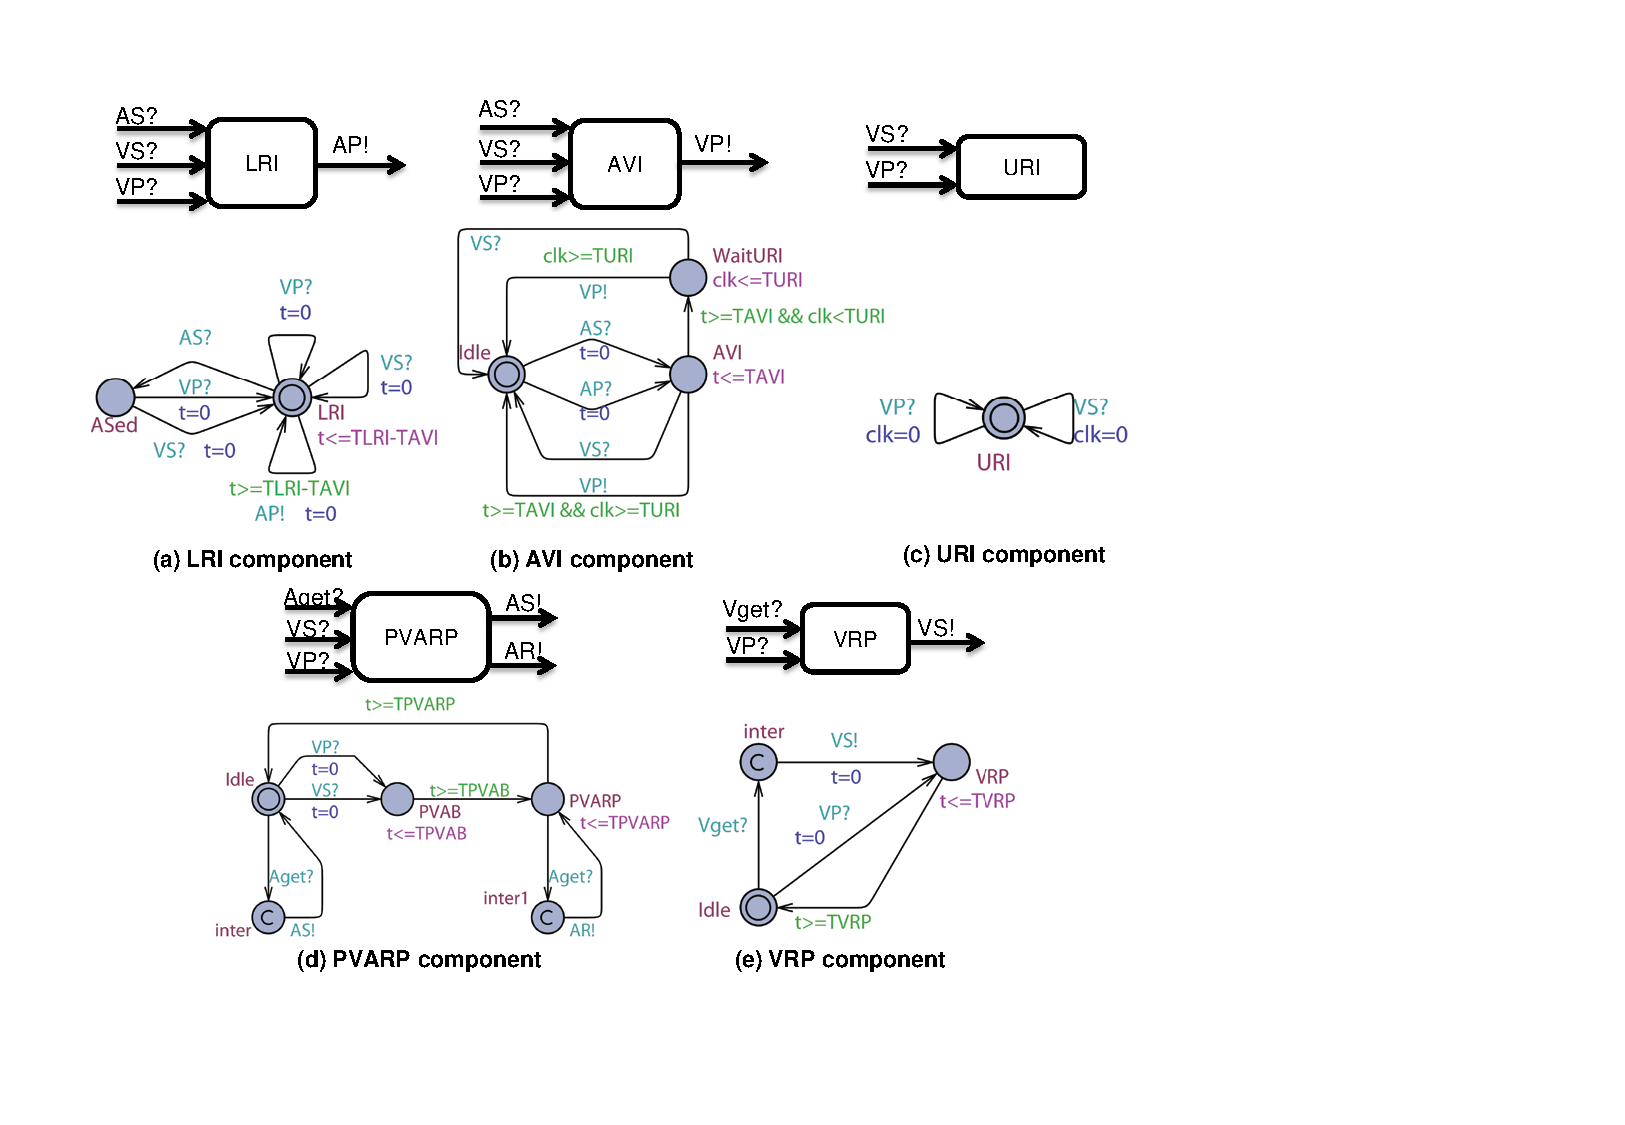
\includegraphics[width=0.9\textwidth]{figs/pacemaker.pdf}
%\vspace{-10pt}
\caption{Five basic timing cycles for a dual chamber pacemaker, which include the Lower Rate Interval (LRI), Atrio-Ventricular Interval (AVI), and Upper Rate Interval (URI). Also included are the blanking intervals, Post Ventricular Atrial Refractory Period (PVARP) and Ventricular Refractory Period (VRP), to inhabit action by the pacemaker.}
\label{fig:PMdesign}
%\vspace{-10pt}
\end{figure} 

\section{Heart Models for Closed-loop Model Checking}
%\begin{itemize}
	%\item What does nondeterminism do? Where can these model be used?
    %\item How to replace complex dynamics of the deterministic models with nondeterminism?
    %\item What are the abstraction rules that can be applied to the heart models and what are their physiological basis?
    %\item How to encode the information loss during each abstraction steps?
%\end{itemize}
During closed-loop model checking, the device model is verified against safety and efficacy properties under physiological conditions covered by the human physiology. 
%The ideal physiological model should be: (1) general enough to cover possible physiological behaviors, and (2) expressive enough to distinguish specific physiological conditions from other conditions. 
%It is obvious that no single model can achieve both properties.
 %A rigorous framework should be adapted so that models with the appropriate level of details are selected.
It is challenging to develop physiological models for closed-loop model checking of autonomous medical devices.
The following aspects need to be taken into account:
\begin{itemize}
\item \textbf{Model Interpretability: } How much detail should the physiological models have in order to unambiguously describe a physiological behavior? In particular, if the model checker returns an execution trace as counter-example, how much detail should the physiological model have so that the execution traces can be interpreted by medical domain experts? 	
	\item \textbf{Behavior Coverage:} What approach must we use for physiological models to cover the large variability of human physiology? How can these models cover rare physiological cases and those that are unknown to us?

	%\hatodoin{what are intermediate states? sentence not clear. }
	\item \textbf{Model Ambiguity: } Multiple physiological conditions can map to the same event trace due to the limited observability of the device. How can we eliminate only the healthy execution from the model so that it would not cause a false-positive?
	\end{itemize}
	The heart model structure proposed in Chapter 3 can be used to model various heart conditions.
	The model structure provides interpretability for closed-loop interaction between the heart and the pacemaker and is capable of solving ambiguities between heart conditions that can map to the same pacemaker execution.
	However, physiological conditions cannot be exhaustively enumerated and model checking on all possible heart models is infeasible.
In the remaining section, over-approximation is first proposed to increase behavior coverage of heart models. 
However, over-approximation inevitably introduces invalid behaviors into the model, which can cause false-positives.
Moreover, due to the loss of details during over-approximation, the interpretability of the model decreases which prevents the model to distinguish between different heart conditions.
At the end of this section, an abstraction tree framework is proposed to balance model abstraction and refinement for closed-loop model checking.
\subsection{Covering More Behaviors With Over-approximation}
Over-approximation \cite{CEGAR} has originally been proposed to reduce model complexity during model checking.
For timed-automata, timed-simulation is a form of over-approximation.
%The most challenging aspect during closed-loop model checking is the abstraction and refinement of the environment model. 
%In \cite{STTT13} we developed a series of heart model abstractions at various abstraction levels. 
%The models are abstracted using abstraction rules derived from physiological knowledge, thus ensuring that each abstraction step covers more physiological conditions. 
%The models in adjacent abstraction levels also satisfy \textsf{timed-simulation} relationship (\cite{simulation}) to ensure complete coverage in the more abstract model. In the remainder of this section, we briefly discuss this multi-scale modeling process and the domain knowledge used. 

For two timed automata $T^1=\left\langle S^1,S_0^1,\Sigma^1,X^1,inv^1,E^1\right\rangle$ and $T^2=\left\langle S^2,S_0^2,\Sigma^2,X^2,inv^2,E^2\right\rangle$, a timed simulation relation is a binary relation $\textsf{sim}\subseteq \Omega^1\times \Omega^2$ where $\Omega^1$ and $\Omega^2$ are sets of states of $T^1$ and $T^2$. We say $T^2$ \textsf{time simulates} $T^1$ ($T^1 \preceq_t T^2$) if the following conditions holds:
\begin{itemize}
	\item Initial states correspondence: $(\left\langle s_0^1,\textbf{0}\right\rangle,\left\langle s_0^2,\textbf{0}\right\rangle)\in \textsf{sim}$
	\item Timed transition: For every $(\left\langle s_1,v_1\right\rangle,\left\langle s_2,v_2\right\rangle)\in\textsf{sim}$, if $\left\langle s_1,v_1\right\rangle\xrightarrow{\delta}\left\langle s_1,v_1+\delta\right\rangle$, there exists $\left\langle s_2,v_2+\delta\right\rangle$ such that $\left\langle s_2,v_2\right\rangle\xrightarrow{\delta}\left\langle s_2,v_2+\delta\right\rangle$ and \\$(\left\langle s_1,v_1+\delta\right\rangle,\left\langle s_2,v_2+\delta\right\rangle)\in\textsf{sim}$.
	\item Discrete transition: For every $(\left\langle s_1,v_1\right\rangle,\left\langle s_2,v_2\right\rangle)\in\textsf{sim}$, if $\left\langle s_1,v_1\right\rangle\xrightarrow{\sigma}\left\langle s_1',v_1'\right\rangle$, there exists $\left\langle s_2',v_2'\right\rangle$ such that $\left\langle s_2,v_2\right\rangle\xrightarrow{\sigma}\left\langle s_2',v_2'\right\rangle$ and $(\left\langle s_1',v_1'\right\rangle,\left\langle s_2',v_2'\right\rangle)\in\textsf{sim}$.
\end{itemize}

Certain properties are preserved for timed simulation relation. 
For $\varphi\in ATCTL$, if $M\preceq_t M'$, we have $M'\models \varphi\Rightarrow M\models\varphi$ \cite{simulation}. 
However, $M'\not\models \varphi\Rightarrow M\not\models\varphi$ does not hold. 
Violations of $ATCTL$ yield \textsf{counter-examples} and the validity of which need to be checked.

In this work, the property of introducing additional behaviors is used as our advantage to cover more behaviors into a more abstract heart model.
By applying physiological abstraction rules to heart models, we creates over-approximation of the heart models that not only covers all behaviors of the original heart model, but also covers additional behaviors that belong to other heart conditions.

It is known that timed simulation relation is also closed under composition \cite{simulation}. 
So when we have two heart models $H_1\preceq_t H_2$ we will have $H_1\| P\preceq_t H_2\| P$ where $P$ is the timed-automata model of the pacemaker. 
For $\varphi\in ATCTL$, we have $H_2\| P\models\varphi\Rightarrow H_1\| P\models\varphi$. 
%With this property we can verify the pacemaker model with abstract heart model. 
%In the rest of the section, we will describe how we develop our initial heart model from the physiological perspective and abstract the model step by step so that the complexity of the model is reduced for verification. 
%Given two heart models $H_1$, $H_2$ and a timed simulation mapping \textsf{sim}=$\Omega_1\times\Omega_2$, there are no automated methods to check $H_1\preceq_t H_2$. In the Appendix, we show the manual proof for the timed simulation relation between two heart models $H_2$ and $H_3$. Other timed simulation relations can be proved similarly.

\subsection{Counter-Example-Guided Abstraction Refinement}
%In closed-loop model checking, there is only one device model. 
%However there can be a large number of environmental conditions which require different models to represent them. For instance, a heart with atrial flutter has an additional conduction pathway that is not present in a healthy heart, causing fast atrial rate. The timing and structural differences of different heart conditions should be distinguished in corresponding heart models.
%%\todo[inline]{should we give an example of a heart condition?}
%A set of initial models of the environment can be constructed but the set is inherently incomplete because of the large number of environment conditions and their combinations. 
%As a result, performing model checking using every model in the set cannot ensure full coverage of the environmental conditions. 
%
%In this paper, domain-specific over-approximation rules are developed that produce abstract models that not only cover explicitly modeled environment conditions, but also cover timing behaviors and conditions not modeled in the set of initial models. 
The abstract heart models obtained by over-approximation can be used for closed-loop model checking of the device model. 
If the closed-loop system satisfies a requirement, the device under verification satisfies the requirement under environment conditions covered by the abstract models. 
However, if the requirement is not satisfied, the model checker returns a counter-example. 
In device modeling, the counter-example is considered \emph{spurious} if it can not be produced by the device (as shown in (\figref{distinction}(a)).
However in environment modeling, even if the counter-example can not be produced by any of the initial environment models, it might still be a physiologically valid behavior.
Thus the validity of a counter-example cannot be determined by refining the environment model, but can ultimately only be determined by domain experts. 

Counter-examples returned from abstract models can be difficult to interpret by domain experts.
One abstract counter-example could be produced by multiple physiologically valid conditions, which causes ambiguity.
Thus, a rigorous framework is necessary to balance the need to cover a wide range of environmental conditions and the need to provide counter-examples to the physicians within their physiological context.

Another challenge for closed-loop model checking of medical devices is the amount of domain expertise needed during: 1) physiological modeling, 2) model abstraction and refinement, and 3) checking the validity of counter-examples.
Thus the framework must also allow non-domain experts to perform verification (item 2 above),
and establish `hand-off' points where the results of verification can be handed back 
to the experts for interpretation.

\begin{figure}[!t]
		\centering
		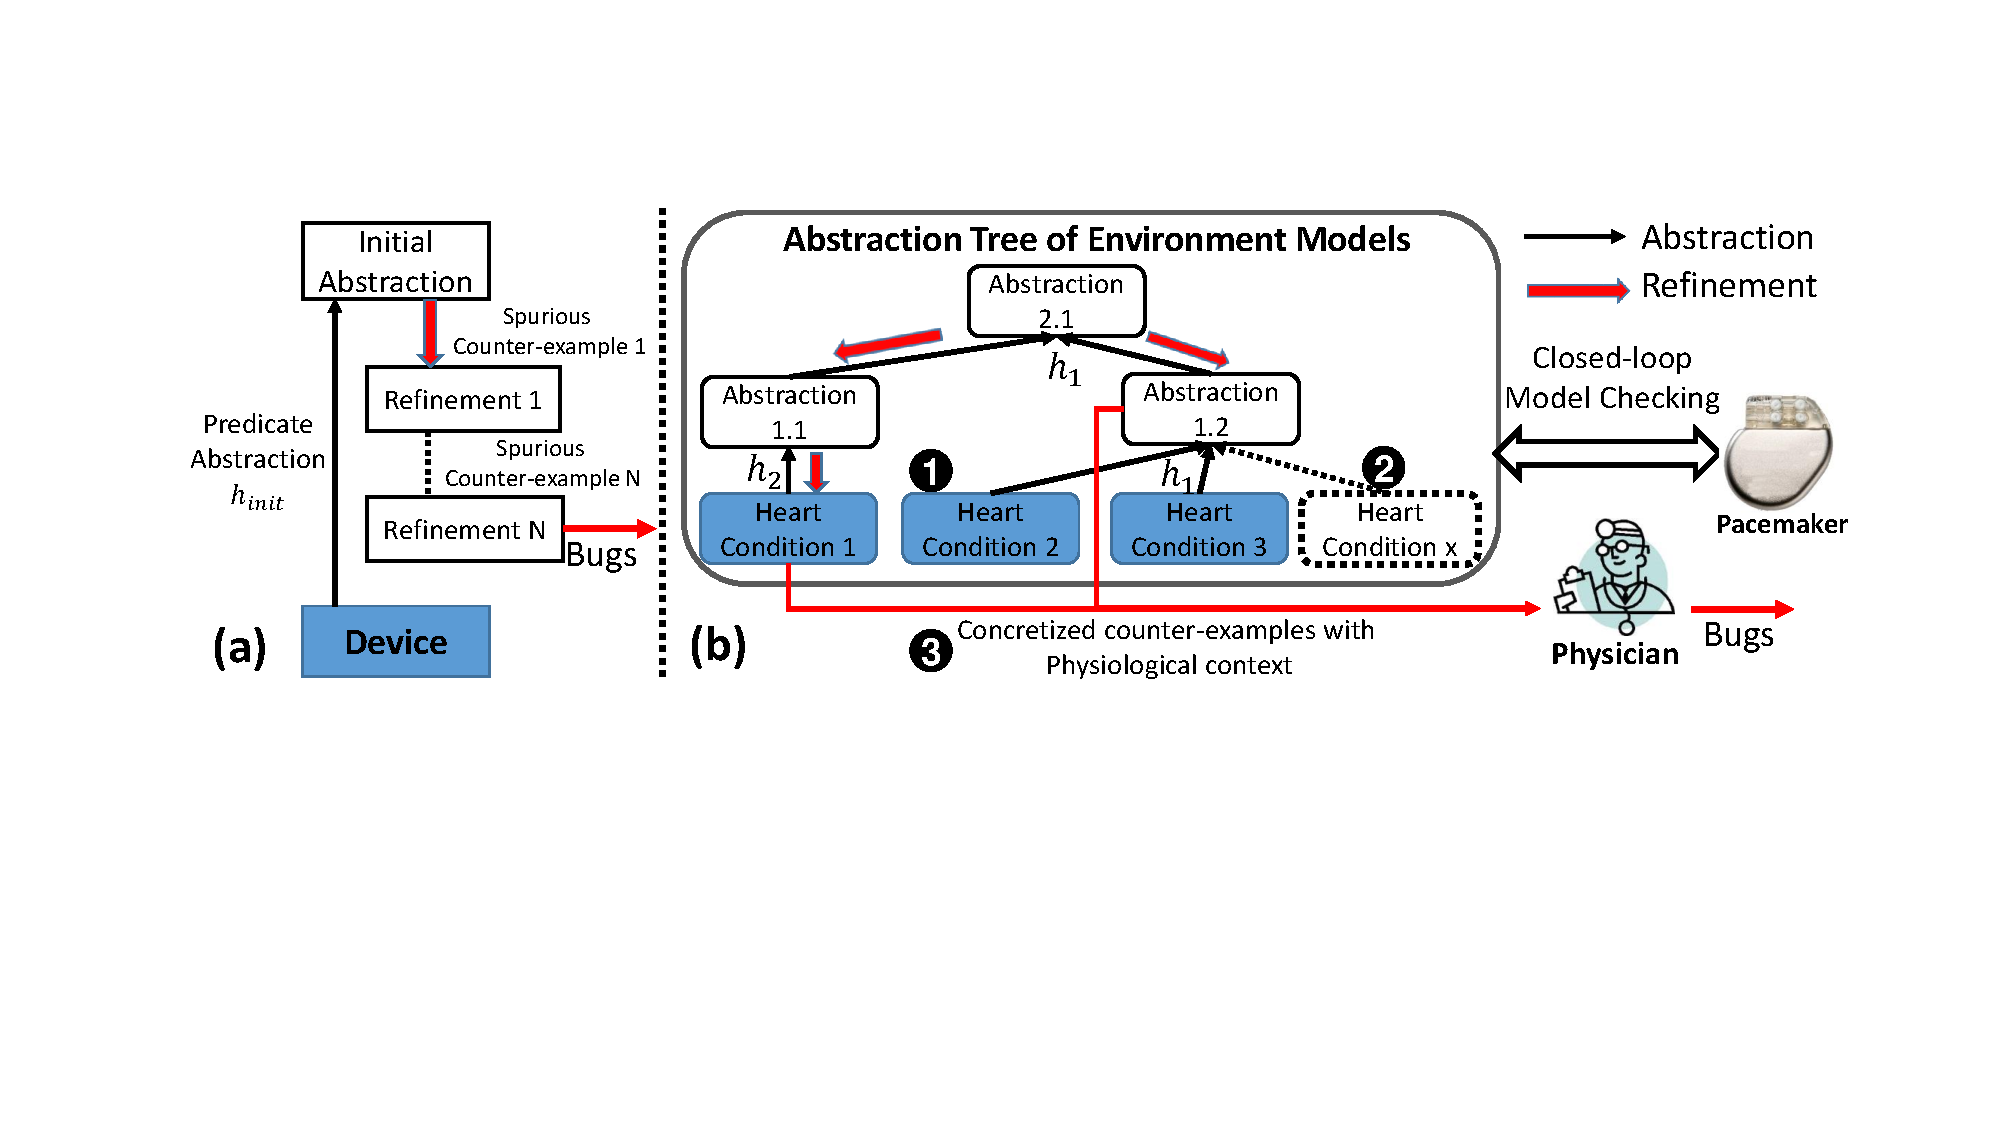
\includegraphics[width=\textwidth]{figs/distinction.pdf}
		%\vspace{-5pt}
		\caption{\small (a) Device modeling with CEGAR framework (b) Closed-loop model checking with environment abstraction tree.}% The initial set of heart conditions are first abstracted and/or merged using abstraction rules $h_1,h_2$ (Marker 1). The abstract model is first used for closed-loop model checking. When a property violation happens, refined models in the abstraction tree are used for model checking. The most concrete counter-examples may be available in the initial model(s) (Marker 2). In the scenario where counter-examples do not exist in explicitly modeled Heart condition 2 and 3, the counter-example in Abstraction 1.2 may correspond to a valid heart condition introduced during abstraction $h_1$. The physician decides the validity of the counter-examples.}
		\label{fig:distinction}
\end{figure}

\subsection{Abstraction Tree for Heart Model Abstraction Refinement}
The ideal heart model for closed-loop model checking of an implantable pacemaker not only covers all possible inputs to the pacemaker, but also has physiological explanations to all known heart conditions.
However, no \textbf{single} heart model can satisfy both requirements.
Therefore, a set of heart models must be employed where the different abstraction levels of the models strike a balance between coverage and expressiveness.
More importantly, the heart models should have rigorous relationships among each other to provide formal guarantees.

In this section we present the abstraction tree framework that maintains formal \emph{Timed Simulation} relationships between heart models and enables automated closed-loop model checking of implantable pacemaker. %\todo{this sentence need revise}
\begin{figure}[!t]
	\centering
	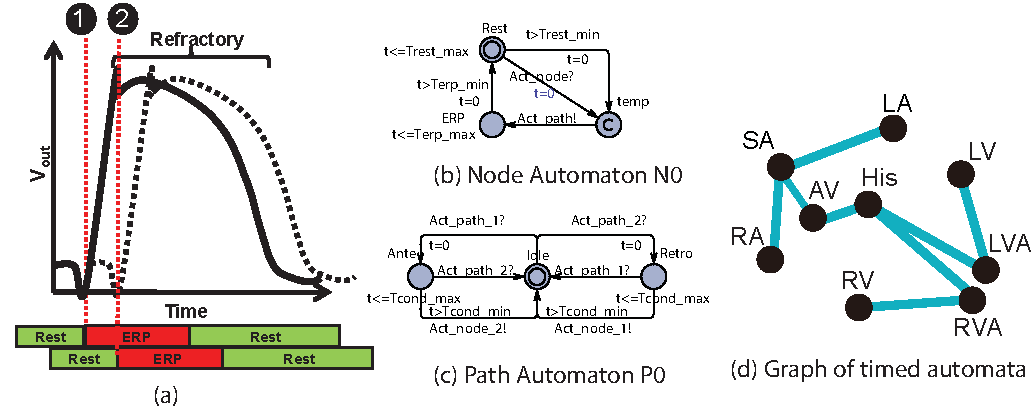
\includegraphics[width=0.9\textwidth]{figs/init_abs.pdf}
	\caption{\small Node and Path Automata which models the timing properties of the heart tissue. A network of node and path automata models the generation and conduction of electrical activities of a heart}
	\label{fig:nodepathTA}
\end{figure}
\subsubsection{Initial Set of Heart Models}
The heart model structure discussed in Chapter 3 is implemented in UPPAAL as shown in \figref{nodepathTA}.
Dynamic changes of the ERP periods and conduction delays are abstracted as ranges using \emph{non-determinism} in timed-automata.
This enables the heart model structure to capture behaviors of the heart models with timing variability.
This heart model structure is based on clinical electrophysiology, with state variables and parameters directly corresponding to physiological parameters.
Therefore, domain experts from clinical electrophysiology can construct models of different heart conditions with their domain expertise and literature.

An example set of initial heart models is shown in \figref{init}.
The different topologies of node and path automata represent the mechanism of different heart diseases.
These heart models represent the current knowledge for heart condition variability, thus the set is inherently incomplete, meaning there is no guarantee for 100\% safety even if a property is satisfied in all of these models.
These models are mostly used for providing physiological contexts for counter-examples returned by the model checker.
Domain experts can always expand the set with knowledge of new heart conditions.
\begin{figure}[!h]
	\centering
	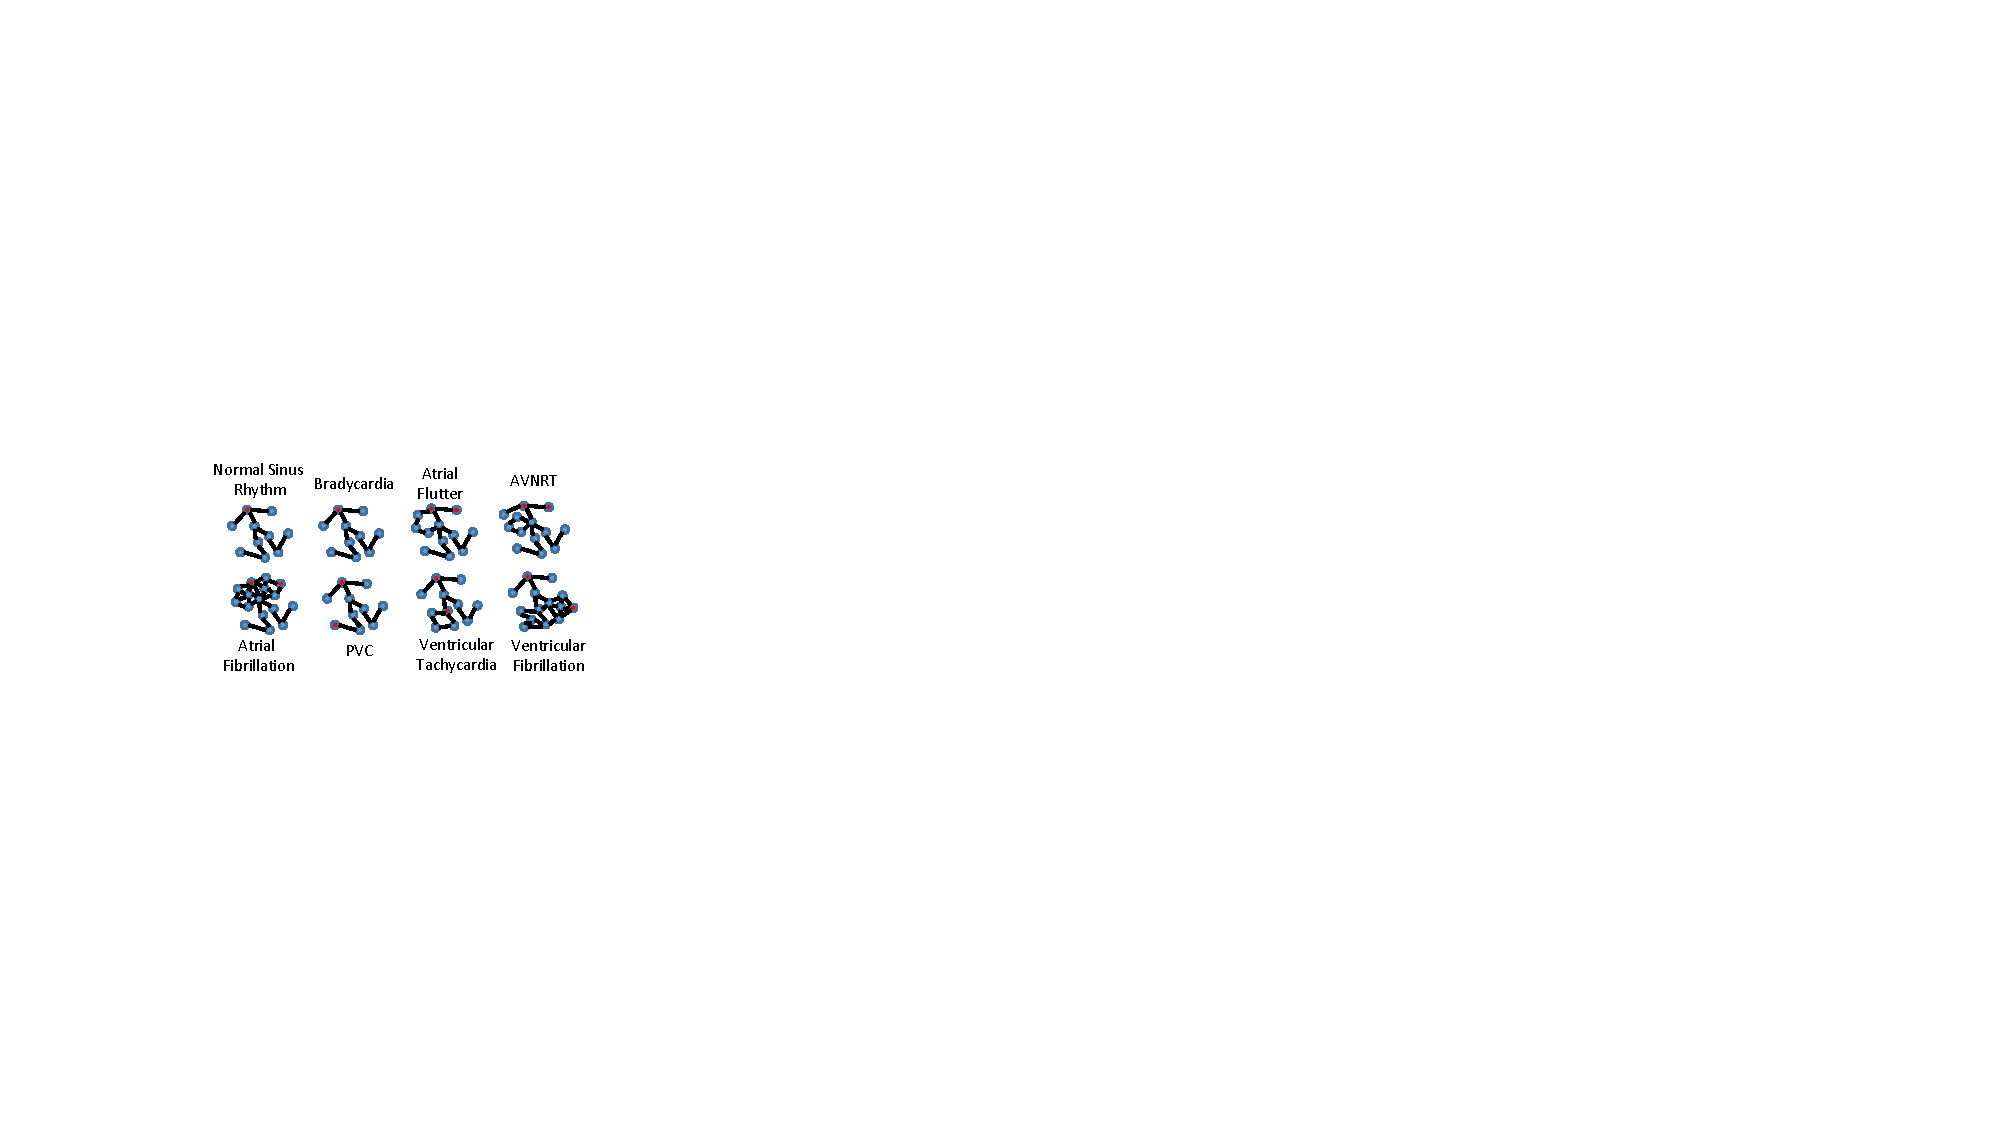
\includegraphics[width=0.8\textwidth]{figs/init.pdf}
	\caption{\small Examples of the initial set of heart models. The models are different in node and path topology and/or timing parameters.}
	\label{fig:init}
\end{figure}
\subsubsection{Interaction With the Pacemaker}
The interactions between the heart and the pacemaker are modeled by using binary event channels. For the atrial lead, we have:
\textsf{$N_A.Act\_path!\rightarrow$Aget!},
and for ventricular lead we have
\textsf{$N_V.Act\_path!\rightarrow$Vget!}.\\
The pacemaker accordingly generates atrial or ventricular pacing actions \textsf{AP!$\rightarrow N_A.Act\_node!$} and \textsf{VP!$\rightarrow N_V.Act\_node!$}.
\subsubsection{Physiological Abstraction Rules}
The initial set of heart models only represents a subset of all possible conditions.
There always exists conditions that are beyond our knowledge or that are combinations of known conditions.
By using \emph{over-approximation}, heart models can be created that cover the observable behaviors of the initial set and that introduce behaviors that were not captured in the initial set.
Inevitably, some of the introduced behaviors will be physiologically invalid.
This problem can be alleviated by carefully designing the abstraction rules so that behaviors introduced are mostly physiologically valid.
The physiologically invalid behaviors can be eliminated during a validity check in the abstraction tree.

Physiological abstraction rules are developed to cover observable behaviors of heart models.
Applying one abstraction rule to heart model(s) $H_1,H_i\dots H_n, n\geq 1$ yields an abstract heart model $H'$ such that all observable behaviors of $H_i$ are covered by $H'$.
For each heart model $H_i$, $H'$ is a \emph{timed simulation} of $H_i$.
To illustrate, a subset of abstraction rules is described intuitively.
The complete set of abstraction rules and the proofs of timed simulation relationship can be found in the tech report \cite{regar_tech}.
%Domain-specific abstraction rules are developed that can introduce new behaviors to a given heart model or a set of models. 
%These new behaviors are physiologically meaningful and might be manifested by a heart condition not explicitly modeled in the initial set of models.
%The physician (or domain expert) remains the ultimate arbiter of what is physiologically meaningful.
%This is a peculiarity of environment modeling, borne out of the fact that the initial set of models is necessarily incomplete, and does not represent all valid behaviors.

%\begin{figure*}[!t]
	%\centering
	%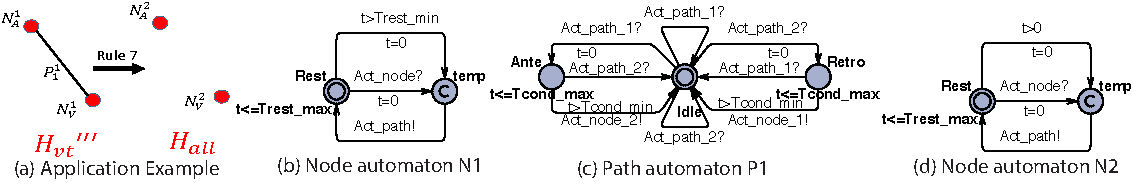
\includegraphics[width=1.05\textwidth]{figs/rule5.pdf}
	%%\vspace{-5pt}
	%\caption{\small (a) Rule 7 application example; (b)(c) Node and path automata used in $H_{vt}'''$; (d) Node automata used in $H_{all}$ }
	%\vspace{-15pt}
	%\label{fig:rule5}
%\end{figure*}
\subsubsection{Rule R1: Convert Reentry Circuits to Activation Nodes}
Within the conduction network of the heart, there can be multiple pathways between two locations, forming conduction loops. If the timing parameters of the tissue along the loop satisfy certain properties, there can be scenarios in which a depolarization wave circling along the circuit. 
The circuits are referred to as \emph{Reentry Circuits}. 
Since the time interval for an activation wave to circle a reentry circuit is usually less than the intrinsic heart cycle length, the heart rate will be "`hijacked"' by the reentry circuit once the cycling is triggered, causing tachycardia. 
Reentry is the most common mechanism for tachycardia, which can be captured by our heart models that are used in \cite{vhm_embc10}. 

The effect of reentry tachycardia is that activation signals coming out of the circuit with a given cycle length equal the sum of conduction delays along the circuit.
It is therefore reasonable to model a reentry circuit as a self-activation node with the self-activation range equal to the sum of conduction delays. \\
\textbf{Applicable Condition: } The rule only affects the topology of the model, and therefore can be applied without preliminaries.\\
\textbf{Output model: }The "essential structure" of a heart model is the shortest paths (in terms of conduction delay) connecting self-activation nodes and/or sensing nodes. 
First detect all circles in the input graph. For each circle with nodes $N_i,i\in[1\dots n]$ and paths $P_j,j\in[1\dots m]$, remove all "non-essential" nodes and paths, create a node automaton $N_s$ and connect to the nearest sensing node with a path automaton $P_s$.\\
\textbf{Effect on parameters: }For the new node automaton $N_s$, the minimum of the Trest parameter is set to the minimum of the sum of the conduction delays within the reentry circuit, and the maximum is set to infinity\\
\textbf{Effect on behaviors: }The new model captures the behavior of the original model when the reentry circuit is active and inactive. Additionally, the new model captures the behaviors of other heart conditions in which the rate of the reentry circuit is lower.
%we have :
%$$N_s.TERP\_min=min(N_i.TERP\_min), N_s.TERP\_max=max(N_i.TERP\_max)$$
%$$N_s.Trest\_min=\sum P_j.Tcond\_min,N_s.Trest\_max=\sum P_j.Tcond\_max$$
%For the new path automaton $P_s$, assume the shortest path from $N_s$ to the nearest sensing node has paths $P_k,k\in[1\dots p]$, we have:
%$$P_s.Tcond\_min=\sum P_k.Tcond\_min,P_s.Tcond\_max=\sum P_k.Tcond\_max$$

\figref{rule1} shows an example in which a circle is replaced by a self-activation node.
\begin{figure}[!h]
	\centering
	
\includegraphics[width=0.4\textwidth]{figs/rule1.pdf}
	\caption{\small Rule R1: Remove reentry circuits from the model}
	\label{fig:rule1}
\end{figure}
\subsubsection{Rule R2: Remove Non-essential Structures}
After the circles within the topology are removed, the topology of the heart model is in the form of a tree. Since the "non-essential" structures do not affect the activation signals from and/or to the sensing nodes, all the "non-essential" structures can be removed.\\
\textbf{Applicable Conditions: }The rule can only be applied after Rule 1 has been applied.\\
\textbf{Output model: } Trimmed topology with only the essential structure remaining.\\
\textbf{Effects on parameters: } There are no effects on parameters of the node and path automata.\\
\textbf{Effects on behaviors: } Applying this rule does not affect the observable behaviors of the model.

\figref{rule2} shows an example in which non-essential structures are removed.
\begin{figure}[!h]
	\centering
	
\includegraphics[width=0.4\textwidth]{figs/rule2.pdf}
	\caption{\small Rule R2: Remove non-essential structures}
	\label{fig:rule2}
\end{figure}
\subsubsection{Rule R3: Removing Unnecessary Non-self-activation Nodes}
The effect of non-self-activation nodes is blocking electrical events with interval shorter than its ERP period. If the self-activation nodes at both ends of a core path have self-activation interval longer than the maximum ERP period of nodes along the core path, the nodes can be removed.

For a core path from a self-activation node $N_1$ to another core node $N_2$, for any structure $P_1-N_n-P_2$ which $N_n$ is a non-self-activation node, if $N_n.ERP_{max}<min(N_1.Rest_{min},N_2.Rest_{min})$, replace $P_1-N_n-P_2$ with $P_3$ so that:
$$P_3.cond_{min}=P_1.cond_{min}+P_2.cond_{min}$$
$$P_3.cond_{max}=P_1.cond_{max}+P_2.cond_{max}$$
\begin{figure}[!h]
	\centering
	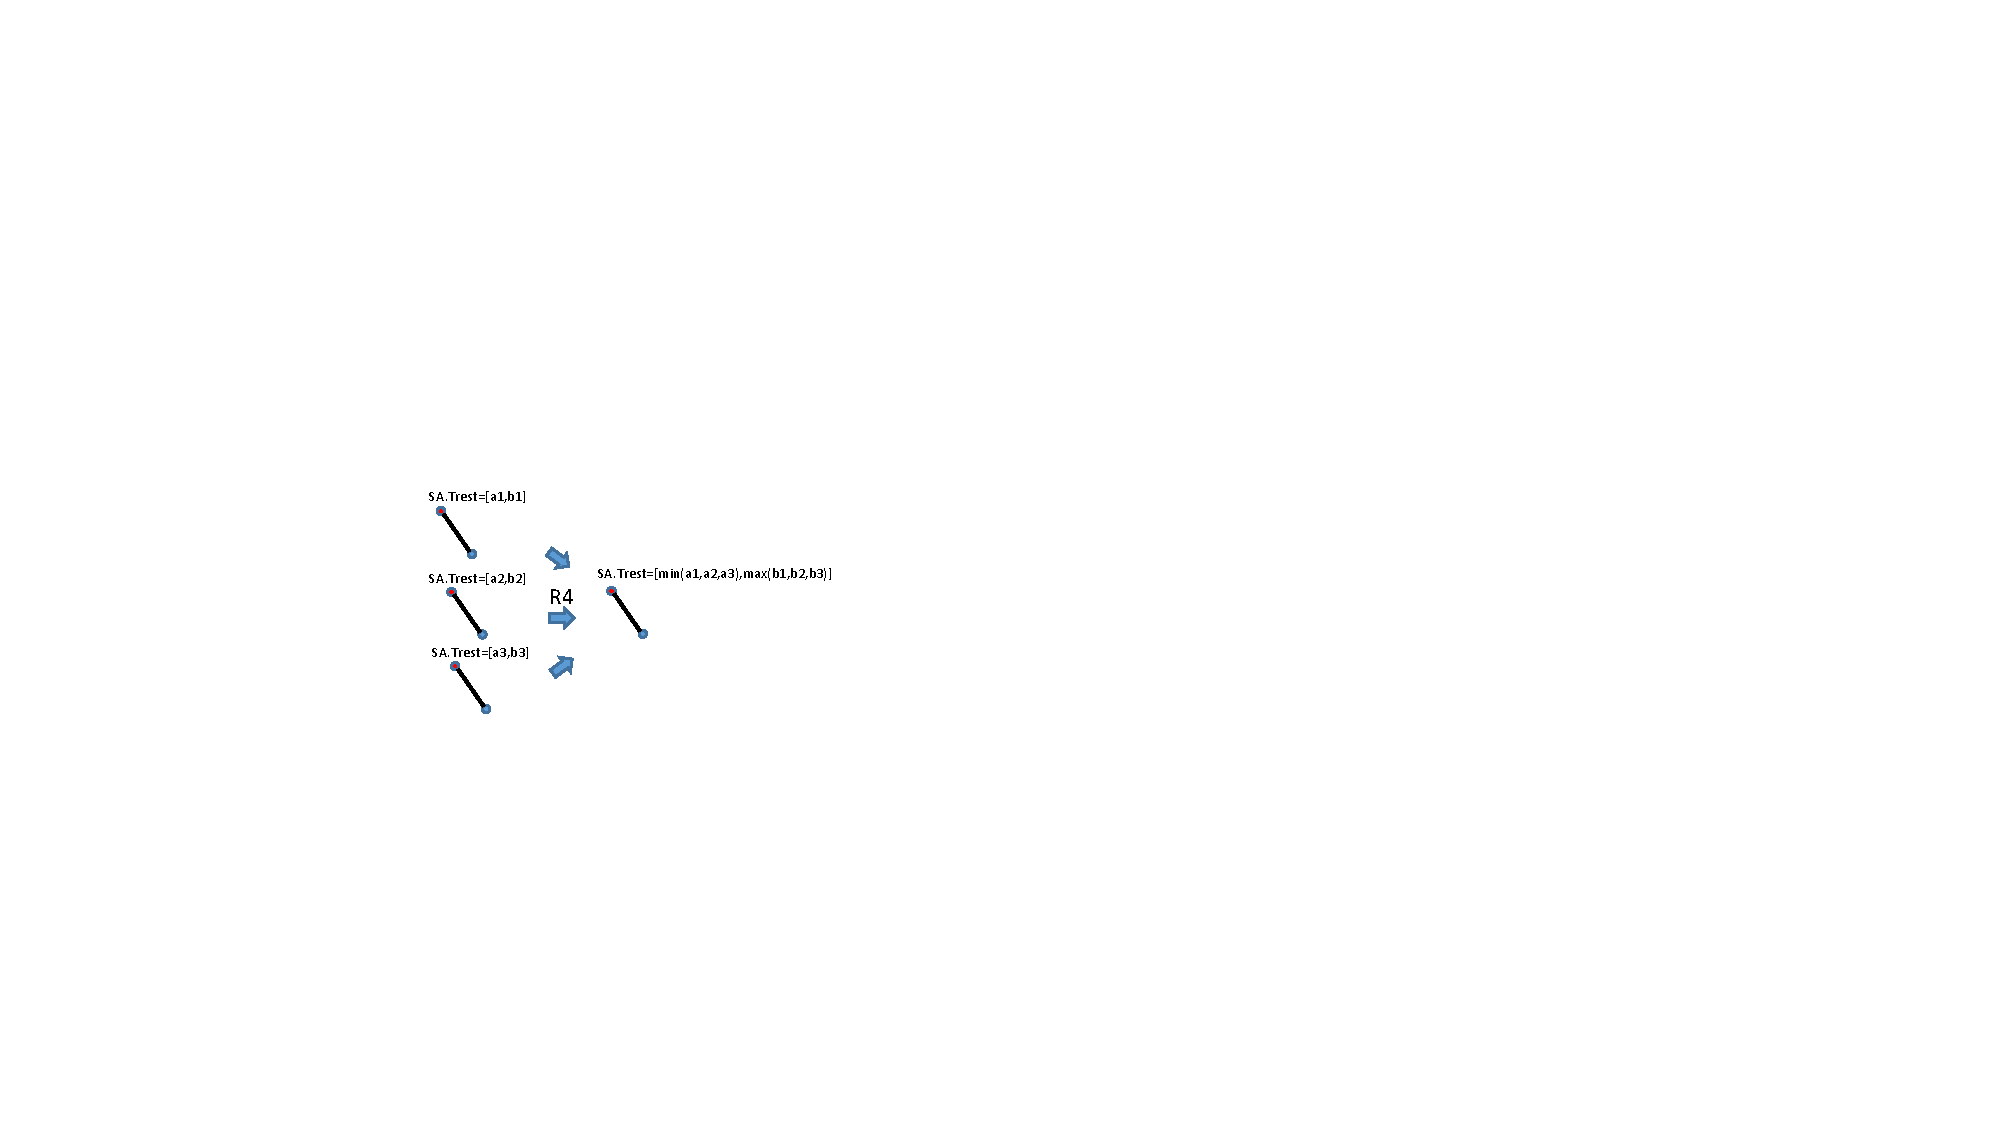
\includegraphics[width=0.7\textwidth]{figs/rule4.pdf}
	\caption{\small Rule R4: Merging parameter ranges}
	\label{fig:rule4}
\end{figure}
\subsubsection{Rule R4: Merge Parameter Ranges}
Timing periods of heart tissue, such as Rest and ERP, are modeled as locations in the node and path automata. 
The minimum and maximum time an automaton can remain in a location is governed by the parameters in the guards and invariants. 
By merging and expanding these periods, new behaviors are introduced where a heart model may remain longer in Rest, activate or self-activate a node faster, andsoforth.
\\
\textbf{Applicable Conditions: }
This rule applies to heart models with the same node and path topology but possibly with different parameters.\\
\textbf{Output Model: }The abstract model has the same topology as the original models.\\
\textbf{Effects on parameters:} The parameter ranges in the new model are a super-set of the parameter ranges in the old models.\\
\textbf{Effects on behaviors: }The abstract model captures all behaviors of the original models. In addition, heart conditions with parameters outside of the ranges of the original models are covered.

\subsubsection{Rule R5: Merge Self-activation Nodes with Interaction Nodes}
%\todo[inline]{not clear}
The effect of self-activation nodes on the interaction of the pacemaker is triggering sensing events within certain delay. In this rule we merge all the self-activation nodes to their neariest interaction nodes. If there exists multiple self-activation nodes merging to the same interaction node, the parameters of the new model are determined following Rule 3.
\begin{figure}[!t]
	\centering
	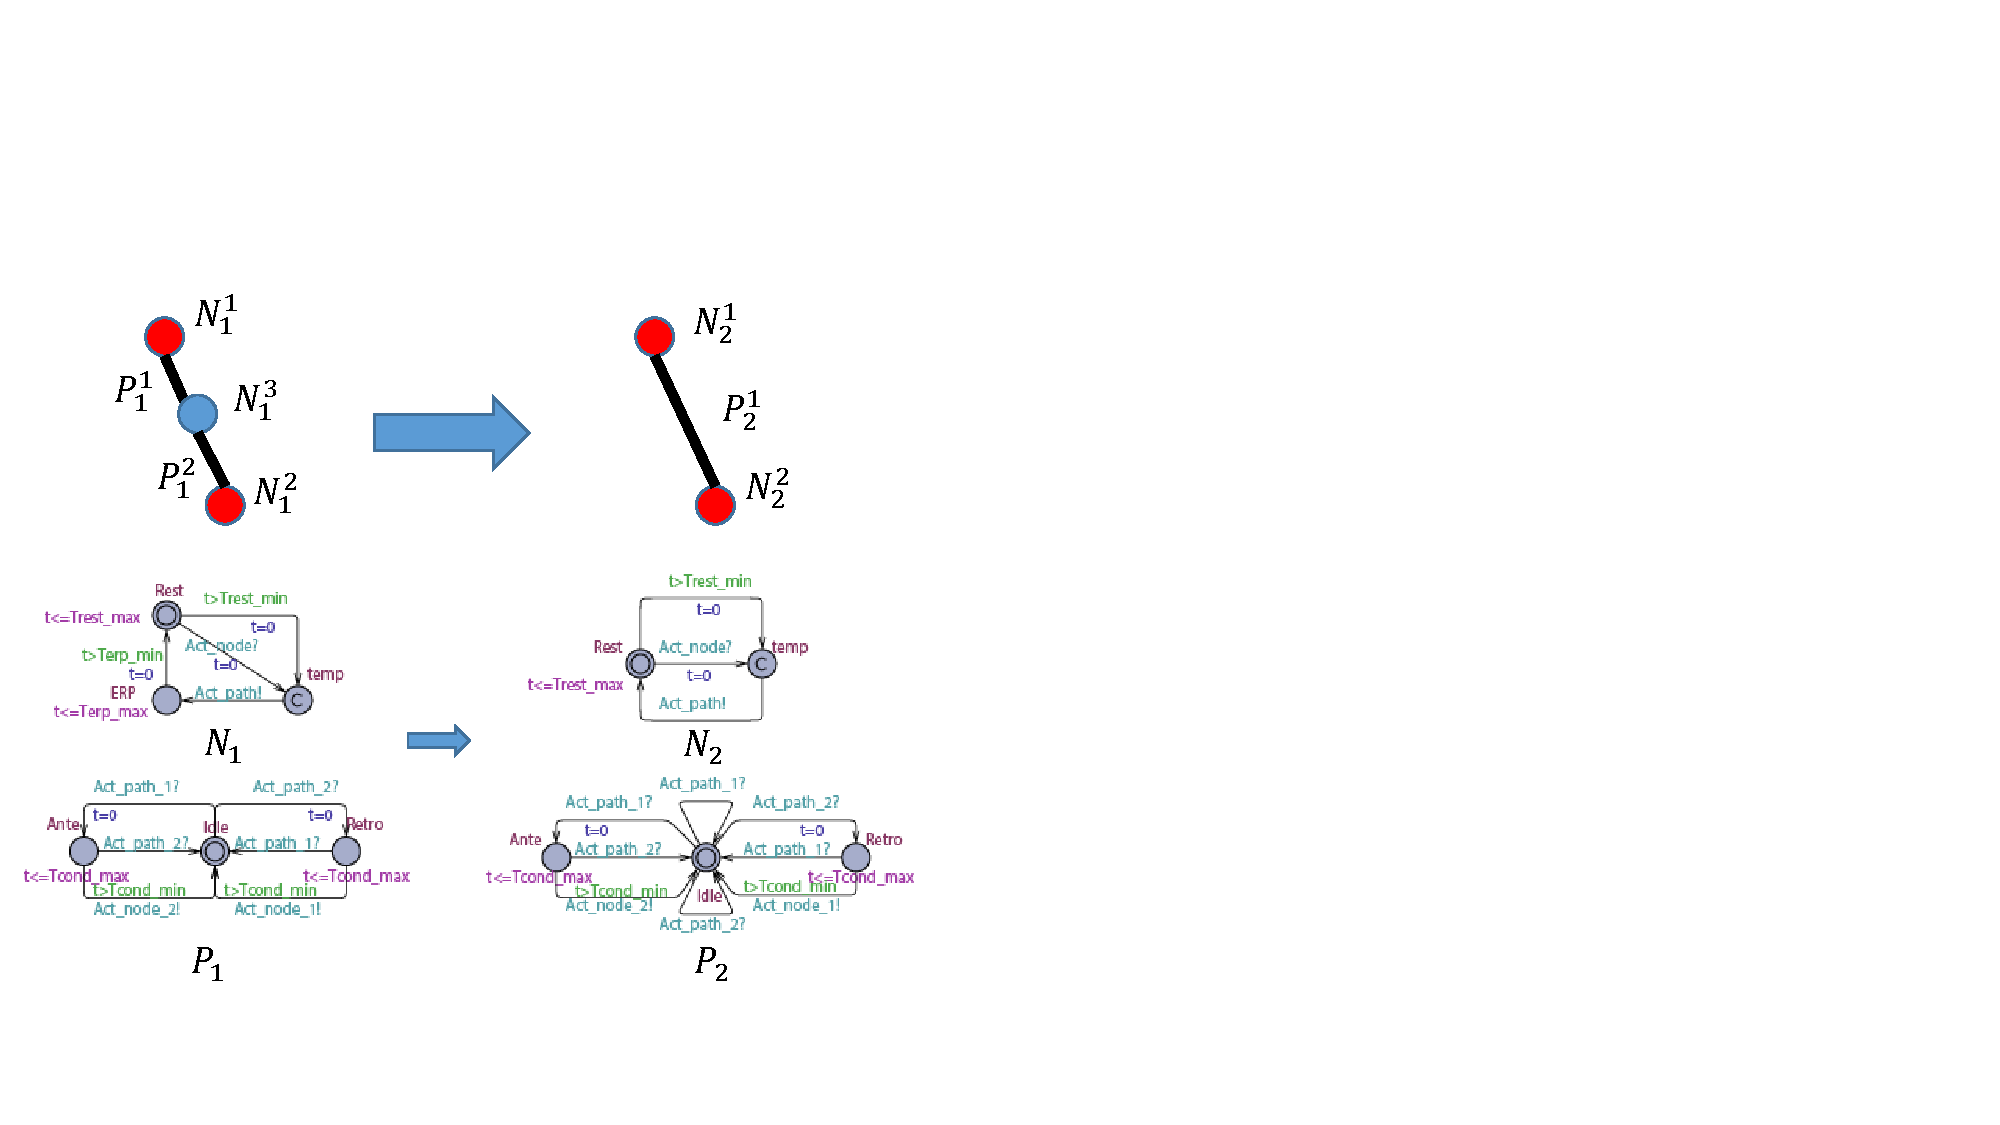
\includegraphics[width=0.8\textwidth]{figs/rule6.pdf}
	%\vspace{-5pt}
	\caption{\small Rule R6 application example: the blocking property of $N_1^3$ is fulfilled by a non-deterministic conduction path $P_2^1$}
	\label{fig:rule6}
\end{figure}
\subsubsection{Rule R6: Replace Blocking With Non-deterministic Conduction}
%\todo[inline]{in modeling section mention self-activating and passive nodes}
%If a node automaton is in its \textsf{ERP} state, a \textsf{Act\_node} event is "blocked" and will not trigger corresponding path conduction. If we add non-deterministic transitions to the path automata such that a \textsf{Act\_path} event do not trigger state transitions to \textsf{ante} or \textsf{retro} (\figref{rule5}), the blocking behavior of the node is covered. We can then merge the \textsf{ERP} state with the \text{Rest} state in the node automata, and all passive nodes can be removed. An application of Rule 6 is shown in \figref{abs_exam}.\\
Consider the structure $N_1^1 P_1^1 N_1^3 P_1^2 N_1^2$ with three nodes and two paths, where $N_1^3$ is a passive node (i.e. not self-activating).
If $N_1^3$ blocks an activation signal from $N_1^1$ to $N_1^2$, this is equivalent to the paths $P_1^1$ or $P_1^2$ not conducting.
In this rule, the structure $P_1^1 N_1^3 P_1^2$ is replaced by a path $P_2^1$ whose automaton can take a self loop when it receives an activation signal, thus effectively stopping the conduction. 
This is shown in Fig.~\ref{fig:rule6}.
Because the blocking effect of nodes is now incorporated into the paths, the node automata of self-activating nodes can be modified to the one shown in Fig.~\ref{fig:rule6}, which does not have the (now useless) ERP period.
\\
\textbf{Subgraph to which it applies}.
Line graphs with 3 vertices $N_1^1 P_1^1 N_1^3 P_1^2 N_1^2$, and self-activating nodes.\\
\textbf{Applicability conditions}.
$N_1^2$ is a passive node.\\
\textbf{Output subgraph}.
$N_2^1 P_2^1 N_2^2$as shown in Fig.~\ref{fig:rule6}\\
\textbf{Effect on parameters}
For the new path, $P.cond_{min}=P_1.cond_{min}+P_2.cond_{min}$ and 
$P.cond_{max}=P_1.cond_{max}+P_2.cond_{max}$
For the new nodes, $N'.Trest_{min}=N.Terp_{min}+N.Trest_{min}$ and 
$N'.Trest_{max}=N.Terp_{max}+N.Trest_{max}$.\\


\begin{figure}[!t]
	\centering
	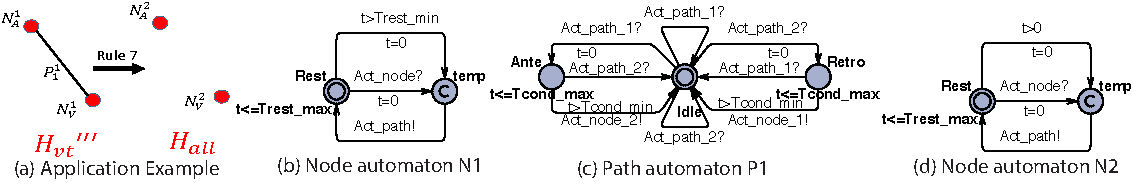
\includegraphics[width=1.05\textwidth]{figs/rule5.pdf}
	%\vspace{-5pt}
	\caption{\small (a) Rule R7 application example; (b)(c) Node and path automata used in $H_{vt}'''$; (d) Node automata used in $H_{all}$ }
	\label{fig:rule5}
\end{figure}

\subsubsection{Rule R7: Replace Conduction With Self-activation}
We describe Rule R7 as it illustrates both effects of an abstraction rule: structure change and modifications to the automata.
The effect of a conduction path is to conduct electrical activity from a node. Since the pacemaker cannot distinguish self-activation of the node and activation triggered by path conduction, we can use self-activation to replace path conduction.
If all self-activation nodes are allowed at any time by setting their minimum Rest period to 0, all the conduction paths can be removed, while preserving the original behaviors (where the Rest period was constrained to a finite interval).\\
\textbf{Applicability conditions}.
This rule can only be applied after Rule 5 and Rule 6 have been applied.\\
\textbf{Output graph}.
All edges are deleted: $G' = (V(G), \emptyset)$. The node automata are replaced with the one shown in \figref{rule5}.d.\\
\textbf{Effect on parameters}
For every node automaton $N$ in $G'$, $N.Trest_{min}=0$.\\

Now we use R7 as example to demonstrate the timed-simulation relationship between heart models before and after the application of R7.
Consider \figref{rule5}.(a) showing an application of R7, $H_{vt}'''=N^1_AP^1N^1_V$ is abstracted to $H_{all}=N^2_AN^2_V$. Here we prove that $H_{vt}'''\preceq_t H_{all}$ with observable events $\Sigma_o=\{N_A.Act\_path,N_V.act\_path\}$. The state of $H_{vt}'''$ is represented by $(N^1_A.loc,P^1_1.loc,N^1_V.loc,N^1_A.t,P^1_1.t,N^1_V.t)$ and the state of $H_{all}$ is represented by $(N^2_A.loc,N^2_V.loc,N^2_A.t,N^2_V.t)$. Due to space limit, only one transition from each category is presented:\\
\textbf{Initial state: }First for the initial state we have:
$$\left\langle (Rest,Idle,Rest,0,0,0),(Rest,Rest,0,0)\right\rangle\in sim_o$$ 
\textbf{Timed transitions: }Consider a timed transition in $H_{vt}'''$
$$(Rest,Idle,Rest,t_1,t_2,t_3)\xrightarrow[]{\tau}(Rest,Idle,Rest,t_1+\tau,t_2+\tau,t_3+\tau)$$
in which $(\tau\in\mathbb{R})\wedge (t_1+\tau\leq N^1_A.Trest\_max)\wedge( t_3+\tau\leq N^1_V.Trest\_max)$. For a state in $H_{all}$ such that $\left\langle (Rest,Idle,Rest,t_1,t_2,t_3),(Rest,Rest,t_1,t_3)\right\rangle\in sim_o$,  there is a timed transition:
$$(Rest,Rest,t_1,t_3)\xrightarrow[]{\tau}(Rest,Rest,t_1+\tau,t_3+\tau)$$
and $\left\langle (Rest,Idle,Rest,t_1+\tau,t_2+\tau,t_3+\tau),(Rest,Rest,t_1+\tau,t_3+\tau)\right\rangle\in sim_o$.\\
%The state of $H_{vt}'''$ is given by the locations of the three automata.
%$$(Rest,Idle,Rest,[Trest\_min, Trest\_max]$$
%$$(Rest,Idle,Rest)\xrightarrow[]{N^1_A.t<N^1_A.Trest\_min \wedge N^1_V.t<N^1_V.Trest\_min}(Rest,Idle,Rest)$$
%are mapped to the following transition in $H_{all}$:
%$$(Rest,Rest)\xrightarrow[]{N^2_A.t<N^2_A.Trest\_min \wedge N^2_V.t<N^2_V.Trest\_min}(Rest,Rest)$$
%
%Self-activations of the atrial node:
%$$(Rest,Idle,Rest,t_1,t_2,t_3)\xrightarrow[\textcolor{red}{N^1_A.Act\_path!}]{t_1\in [N^1_A.Trest\_min, N^1_A.Trest\_max] }(Rest,Ante,0,0,t_3)$$
%are mapped to the following transition in $H_{all}$:
%$$(Rest,Rest,t_1,t_3)\xrightarrow[\textcolor{red}{N^2_A.Act\_path!}]{t_1\in [0, N^2_A.Trest\_max]}(Rest,Rest,0,t_3)$$
%Self-activations of the ventricular node:
%$$(Rest,Idle,Rest,t_1,t_2,t_3)\xrightarrow[\textcolor{red}{N^1_V.Act\_path!}]{t_3\in [N^1_V.Trest\_min, N^1_V.Trest\_max] }(Rest,Retro,Rest,t_1,0,0)$$
%are mapped to the following transition in $H_{all}$:
%$$(Rest,Rest,t_1,t_3)\xrightarrow[\textcolor{red}{N^2_V.Act\_path!}]{t_3\in [0, N^2_V.Trest\_max]}(Rest,Rest,t_1,0)$$
\textbf{Discrete transitions: }Consider a discrete transition in $H_{vt}'''$
$$(Rest,Ante,Rest,t_1,t_2,t_3)\xrightarrow[t_2\in [P^1_1.Tcond\_min, P^1_1.Tcond\_max) ]{\textcolor{red}{N^1_V.Act\_path!}}(Rest,Idle,Rest,t_1,t_2,0)$$
in which $N^1_V.Act\_path!\in\Sigma_o$. \\
For a state in $H_{all}$ such that $\left\langle (Rest,Idle,Rest,t_1,t_2,t_3) ,(Rest,Rest,t_1,t_3)\right\rangle\in sim_o$,  there is a discrete transition:
$$(Rest,Rest,t_1,t_3)\xrightarrow[t_3\in [0, N^2_V.Trest\_max)]{\textcolor{red}{N^2_V.Act\_path!}}(Rest,Rest,t_1,0)$$
and $\left\langle ((Rest,Idle,Rest,t_1,t_2,0)),(Rest,Rest,t_1,0)\right\rangle\in sim_o$. Basically activation due to conduction is replaced by self-activation of the corresponding node automata.\\
\textbf{Additional behaviors: }The timed-simulation also allows additional behaviors into $H_{all}$. Consider a discrete transition in $H_{all}$
$$(Rest,Rest,t_1,t_3)\xrightarrow[t_3\in [0, N^2_V.Trest\_min)]{\textcolor{red}{N^2_V.Act\_path!}}(Rest,Rest,t_1,0)$$
However, for a state in $H_{vt}'''$ such that $\left\langle (Rest,Idle,Rest,t_1,t_2,t_3),(Rest,Rest,t_1,t_3)\right\rangle\in sim_o$, when $t_3\in [0, N^1_V.Trest\_min]$ there is no available discrete transitions. Physiologically, these implicitly included behaviors correspond to fast heart rate, premature heart events and even noise.



\subsubsection{Abstraction Tree}
By applying the abstraction rules to the initial set of heart models, an abstraction tree is created.
\figref{HM_abs} shows an example of an abstraction tree with the root model capturing all possible input sequences to the pacemaker.
Self-activating nodes are marked as red and the Trest parameters are specified next to them.
Note that this abstraction tree is not unique.
With a different initial set of heart models and/or different rule application orders the abstraction tree can be very different.
The abstraction tree can also be extended at any time if new heart conditions are specified.
The following section demonstrates the use of this abstraction tree during the closed-loop model checking of the pacemaker design.

 \begin{figure*}[!t]
	\centering
	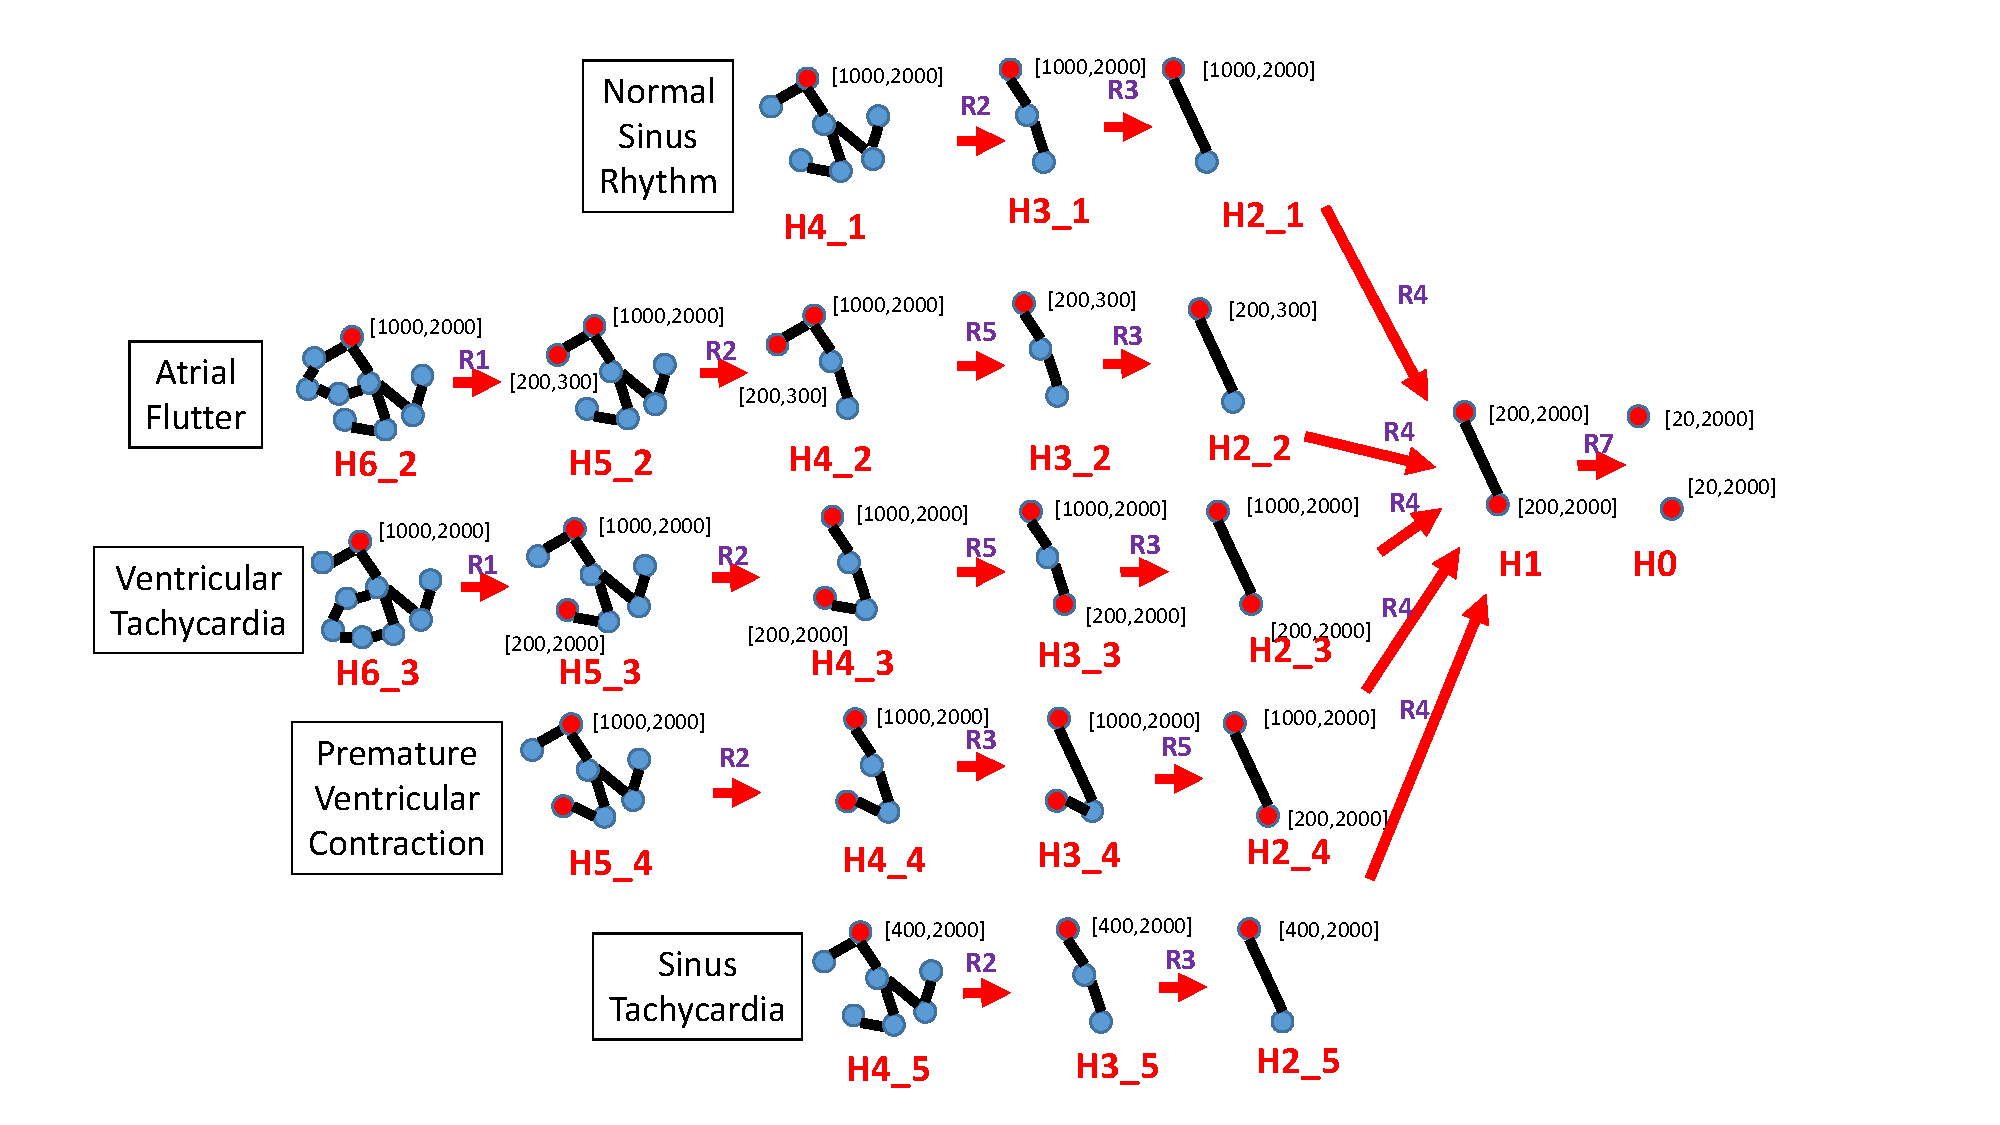
\includegraphics[width=0.95\textwidth]{figs/abs_tree.pdf}
	%\vspace{-5pt}
	\caption{\small One example of abstraction tree of heart models}
	\label{fig:HM_abs}
\end{figure*}


\section{Efficacy Validation for Implantable Pacemaker}
The most essential function for the pacemaker is to treat bradycardia by maintaining the ventricular rate above a certain threshold. We define the region where the ventricular rate is slow, as \textsf{unsafe}. The monitor \textsf{PLRI\_test} is designed to measure intervals between ventricular events and is shown in \figref{safety1}. For property
\begin{center}
\textsf{$\varphi_{LRI}=$A[] (PLRI\_test.secV imply PLRI\_test.t$\leq$TLRI)}
\end{center}
we have a closed-loop system with heart model $H_0$ : 
$$H_0\| P\| PLRI\_test\models\varphi_{LRI}$$

\begin{figure*}[b]
\centering
%\vspace{-10pt}
		\subfigure[Monitor \textsf{PLRI\_test}] {
				\includegraphics[width=0.4\textwidth]{figs/LRI_test.pdf}
				\label{fig:safety1}
		} 
		\subfigure[Monitor \textsf{PURI\_test}] {	
			\includegraphics[width=0.3\textwidth]{figs/uri_test.pdf}
			\label{fig:uri_test}
		}
		%\vspace{-10pt}
	\caption{(a) Monitor for LRL: Interval between two ventricular events should be less than TLRI, (b) Monitor for URL: Interval between a ventricular event and a VP should be longer than TURI}
\end{figure*} 

The pacemaker is not designed to treat tachycardia so it can only pace the heart to increase its rate and cannot slow it down. To mitigate the hazard that the pacemaker may increase the heart rate above physiological need, an Upper Rate Interval (URI) is specified such that the pacemaker can increase the ventricular rate up to this limit. 
  
We require that a ventricle pace (VP) can only occur at least $TURI$ after a ventricle event (VS, VP). The monitor \textsf{PURI\_test} is shown in \figref{uri_test}. For the property
\begin{center}
$\varphi_{URI}=$\textsf{A[] (PURI\_test.secV imply PURI\_test.t$\geq$TURI)}
\end{center}
we have: $$H_0\| P\| PURI\_test\models \varphi_{URI}$$

As we saw in the above examples, the efficacy requirements are satisfied with the most abstract heart model.
Therefore no heart model refinements are necessary and the requirements are satisfied under all possible heart conditions.

%\section{Evaluate the Mitigation}
%As described in Chapter \ref{Mode_switch}, the mode switch algorithm has been designed to mitigate the hazard that the A-V synchrony function of DDD pacemaker extends fast
%atrial rate to the ventricle. It is important to ensure the effectiveness of the algorithm without inducing other top-level hazards. In this section we first show the existence of the hazard in a pacemaker without the mode-switch algorithm. If the algorithm if effective the hazard will not exist after introducing the algorithm.
%
%\subsection{Existence of Pacemaker Mediated Tachycardia during SVT}
%The monitor \textsf{Pv\_v} is designed to show existence of PMT during SVT. It goes to the error state if the ventricular rate drops below the Upper Rate Limit (\figref{vv}).  
%
%
%We specify 
%$\varphi_{MS}=E[] (not Pv\_v.err)$\\
%which verifies the existence of PMT. The heart model $H_e$ in Fig. \ref{fig:HM_abs} is not suitable for this property since the non-deterministic conduction of component $P_3$ does not capture the blocking property of the AV node, which is the key in PMT. We use a more refined model $H_d$ which has AV node modeled. To identify the PMT scenario, we first set $H_d.N^1.Trest\_min<100$ so that the atrial rate can be high and $H_d.N^2.Trest\_min>TURI$ so that the intrinsic heart rate is less than TURI. The property is first verified on pacemaker without the mode-switch algorithm. We have $H_d\|P\|Pv\_v\models\varphi_{MS}$ and the evidence returned by the model checker illustrates the PMT scenario.
%
%% There are two separate AVI and LRI components for each mode and switches to the corresponding ones when synchronization signals are received. The clock values are kept so that essential intervals are kept. 
%\subsection{Verification against fundamental safety properties}
%For a pacemaker with the mode switch algorithm: 
%
%$P_2$=\textsf{LRI'$\|$AVI'$\|$URI$\|$PVARP$\|$VRP$\|$INT$\|$CNT$\|$DUR}, 
%
%we verify the same fundamental safety properties on the pacemaker model with mode-switch algorithm. We have:
%$$H_d\|P_2\|PURI\_test\models\varphi_{URI}$$
%$$H_d\|P_2\|PLRI\_test\not\models\varphi_{LRI}$$


\section{Safety Validation for Implantable Pacemaker}
A dual chamber pacemaker is designed to increase the heart rate during bradycardia, but it should also not increase the heart rate inappropriately.
Inappropriate increase of heart rate by the pacemaker is referred to as \emph{Pacemaker Mediated Tachycardia (PMT)}.
Previous work \cite{STTT13} used model checking to identify two known PMT conditions.
However, in order to avoid ambiguities in the counter-examples, the properties for the two PMTs were specified very specifically, which abandoned the advantage of model checking to find unknown safety violations.

With the abstraction tree approach, the ambiguities can potentially be resolved since the abstraction tree considers all known heart conditions.
Therefore the property for PMTs can be specified more generally.
In this paper, we specify a property such that\\
$\varphi_{PMT}$: \emph{The interval between ventricular events (Vget, VP) should not be shorter than TURI for 30 consecutive beats}\\
which means that the ventricular rate should not be faster than the upper rate interval (TURI) for too long, either intrinsically or because of pacemaker interaction.
Counter-example because of intrinsic fast ventricular rates can be removed from results after analysis from the abstraction tree.

A UPPAAL monitor $M_{con}$ for the property is shown in Fig. \ref{fig:monitor}, and the TCTL property is specified as:\\
\begin{center}
\emph{A[] not $M_{con}$.err}
\end{center}

\begin{figure}[!t]
	\centering
	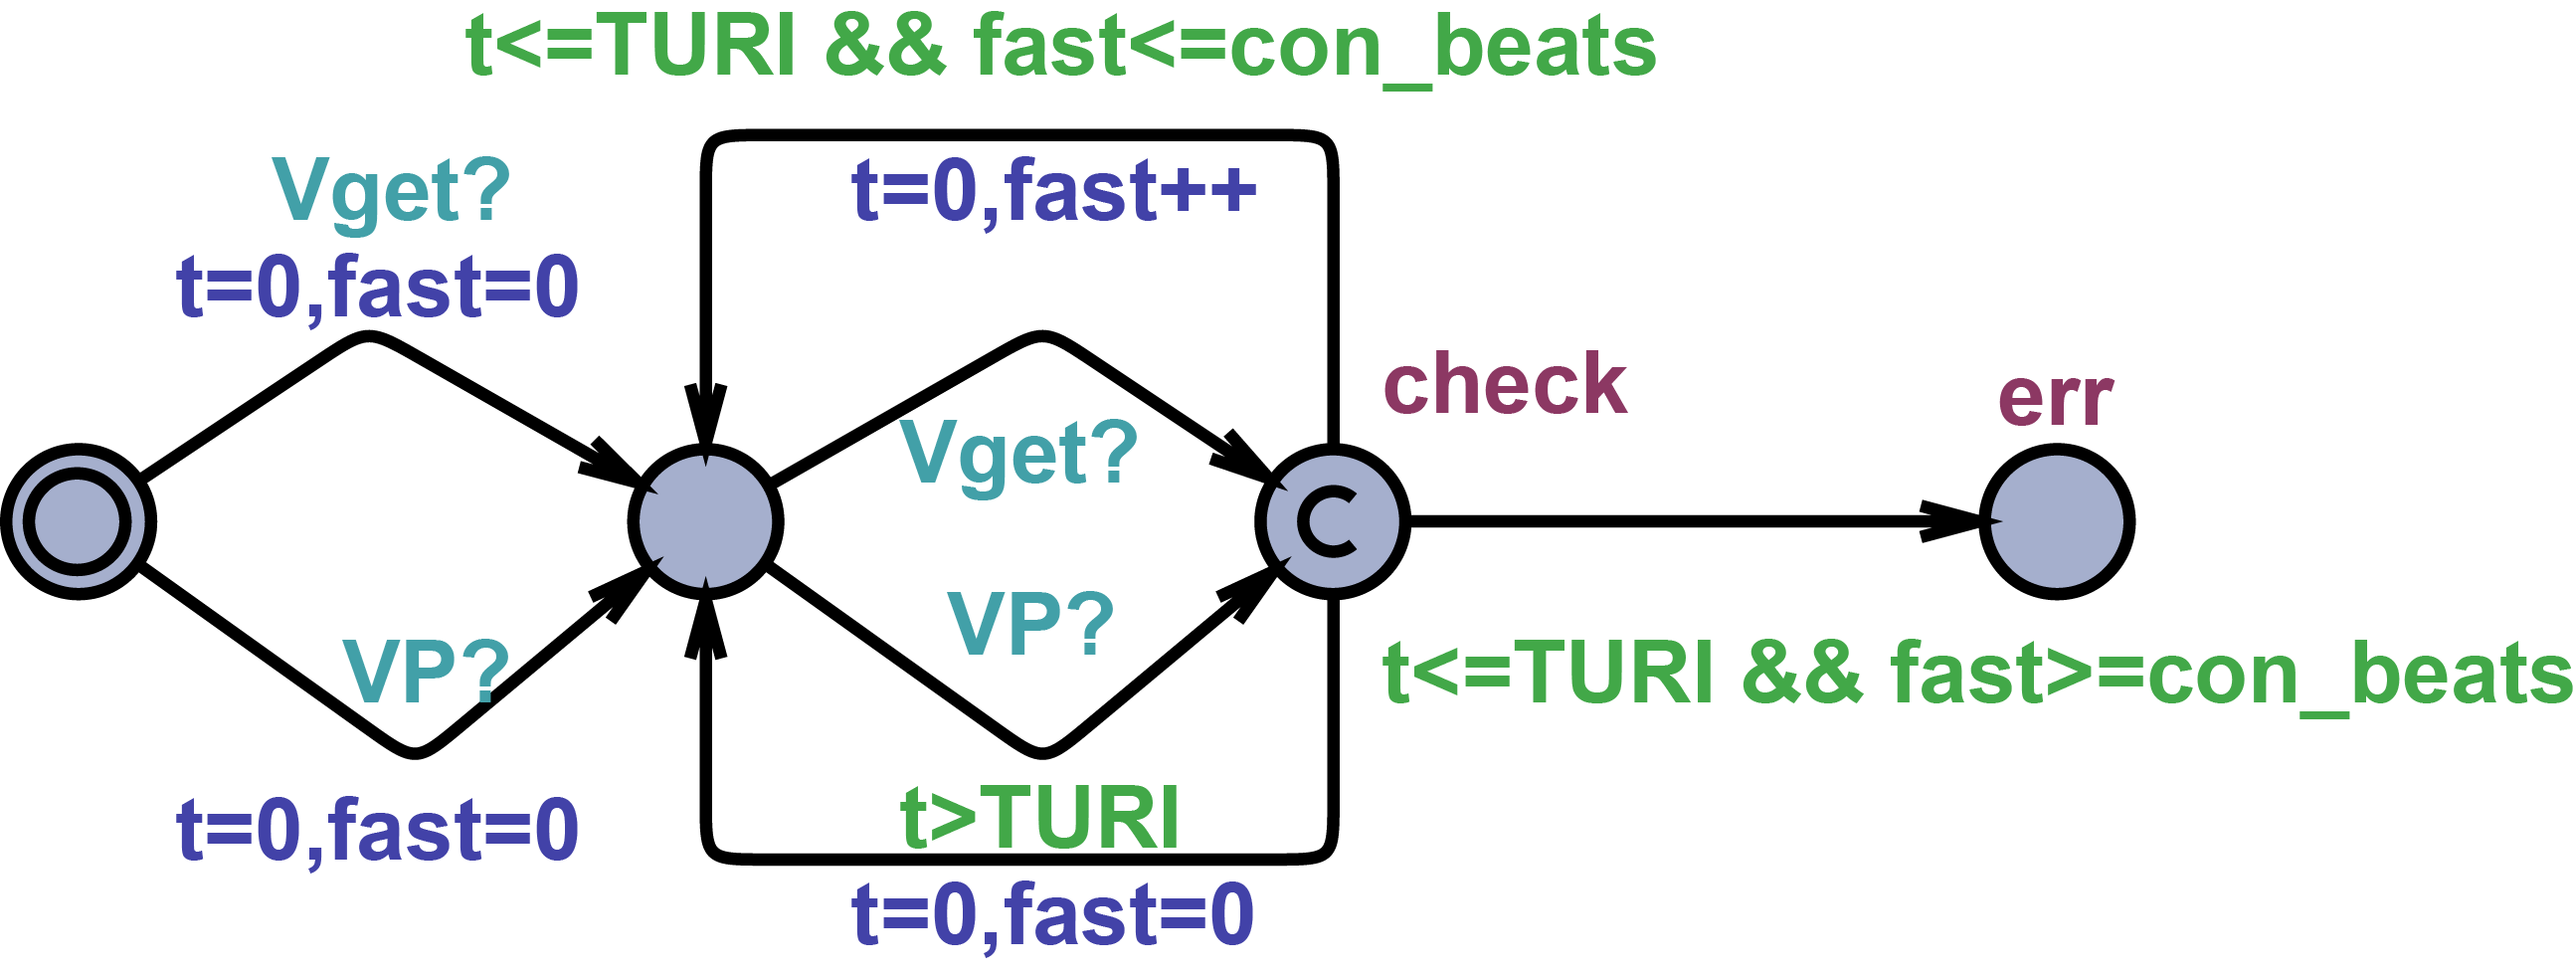
\includegraphics[width=0.4\textwidth]{figs/monitor.png}
	\caption{\small UPPAAL monitor for Property 1}
	\label{fig:monitor}
\end{figure}

The model checker UPPAAL was used to check Property $\varphi_{PMT}$ on the pacemaker model using the abstraction tree of heart models.
The property is violated in $H0 || PM$, thus thus the abstraction tree is followed to select pair $H1$ with the pacemaker model and Property 1 is verified again.
The process continues till either the leaves of the tree are reached of the property is satisfied.
The result is shown in \figref{CE}, which demonstrates 5 different scenarios that can happen when using the abstraction tree.
The shaded area marks the heart models with counter-examples.
\begin{figure*}[!t]
	\centering
	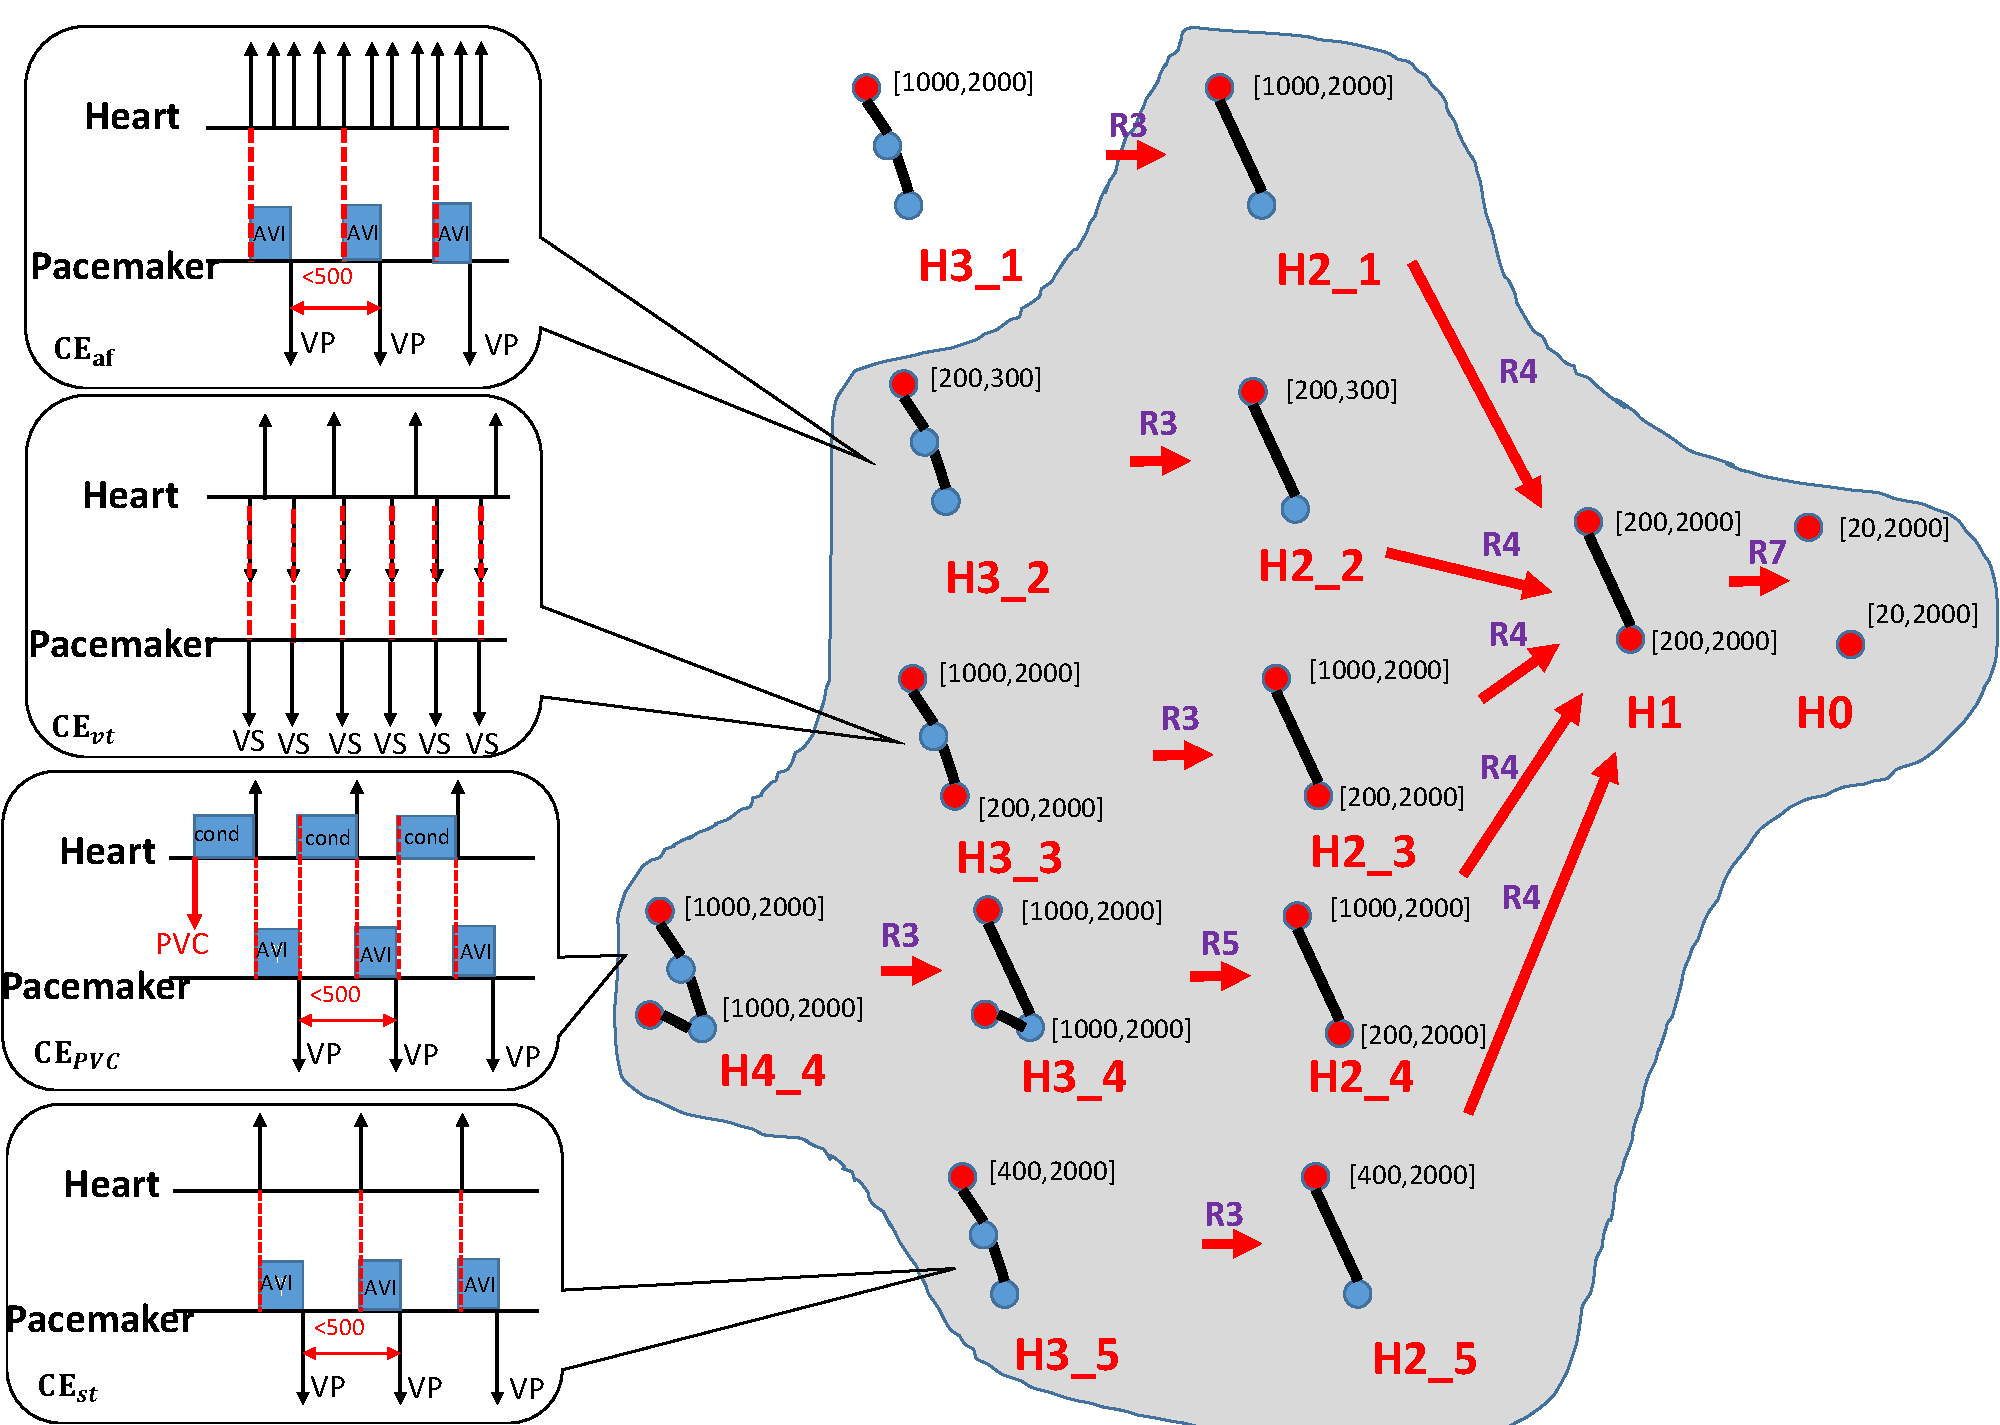
\includegraphics[width=0.8\textwidth]{figs/tree.pdf}
	%\vspace{-5pt}
	\caption{\small Four different physiological conditions in which Property 1 is violated. In $CE_{af}$ the pacemaker extends a fast atrial rate to a dangerously fast ventricular rate; in $CE_{vt}$ the ventricular rate is intrinsically fast; in $CE_{st}$ the pacemaker appropriately maintained A-V conduction delay; in $CE_{pvc}$ the pacemaker inappropriately increased the ventricular rate, causing Endless Loop Tachycardia}
	\label{fig:CE}
\end{figure*}

\textbf{Case 1:} Property 1 is violated in $H2\_1 || PM$ but is satisfied in its children $H3\_1 || PM$.
Careful examination of the counterexample finds it to be spurious and so it is successfully eliminated by model refinement.

\textbf{Case 2:} $CE_{af}$ is returned by $H3\_2 || PM$ and corresponds to intrinsic atrial tachycardia with fast atrial rate, which is a sub-optimal but non-lethal condition.
The AV node of the heart will block a subset of the electrical events and maintain a normal ventricular rate.
However, despite the filters in the pacemaker, the pacemaker still paces the ventricle for every 3 atrial activations, which extends fast atrial rate to more dangerous fast ventricular rate. 
The condition is referred to as Atrial Tachycardia Response in which the ventricular rate is increased inappropriately, thus requires revision of the pacemaker design.

\textbf{Case 3:} $CE_{vt}$ is returned by $H3\_3 || PM$ and corresponds to intrinsic ventricular tachycardia with fast ventricular rate.
The counter-example is physiologically valid but the fast ventricular rate is due to the heart itself and is beyond pacemaker functionality.
Therefore this scenario demands no revision of the pacemaker design.

\textbf{Case 4:}  $CE_{st}$ is returned by $H3\_5 || PM$ and corresponds to sinus tachycardia, for instance, when the patient is exercising.
The pacemaker improved the open-loop heart condition by pacing the ventricles $AVI$ after each atrial event, which is a correct operation of the pacemaker despite the requirement violation. 

\textbf{Case 5:} $CE_{pvc}$ is returned by $H4\_4 || PM$ and has a very similar input-output relationship to $CE_{n}$. 
However, the activations of the atrial node are triggered by retrograde conduction from ventricular paces (marker \textsf{cond}). 
The atrial activations trigger another ventricular pace after $AVI$, which will trigger another retrograde conduction. In this case the heart rate is inappropriately high, which corresponds to a dangerous closed-loop behavior referred to as \emph{Endless Loop Tachycardia}.

From the above result, it can be seen that abstraction tree is able to 1) refine a heart model to eliminate spurious counter-examples as in Case 1; 2) provide (multiple) physiological explanations to a counter-example as in Case 2-5; and 3) resolve ambiguities caused by abstraction as in Case 4 and 5.

Device manufacturers have developed algorithms aiming to eliminate behaviors showed in Case 2 and Case 5.
In the following section we demonstrate the use of abstraction tree to evaluate the effectiveness of these algorithms.

\subsection{Terminating Endless Loop Tachycardia}


%\begin{figure*}
		%\centering
		%%\vspace{-20pt}
		%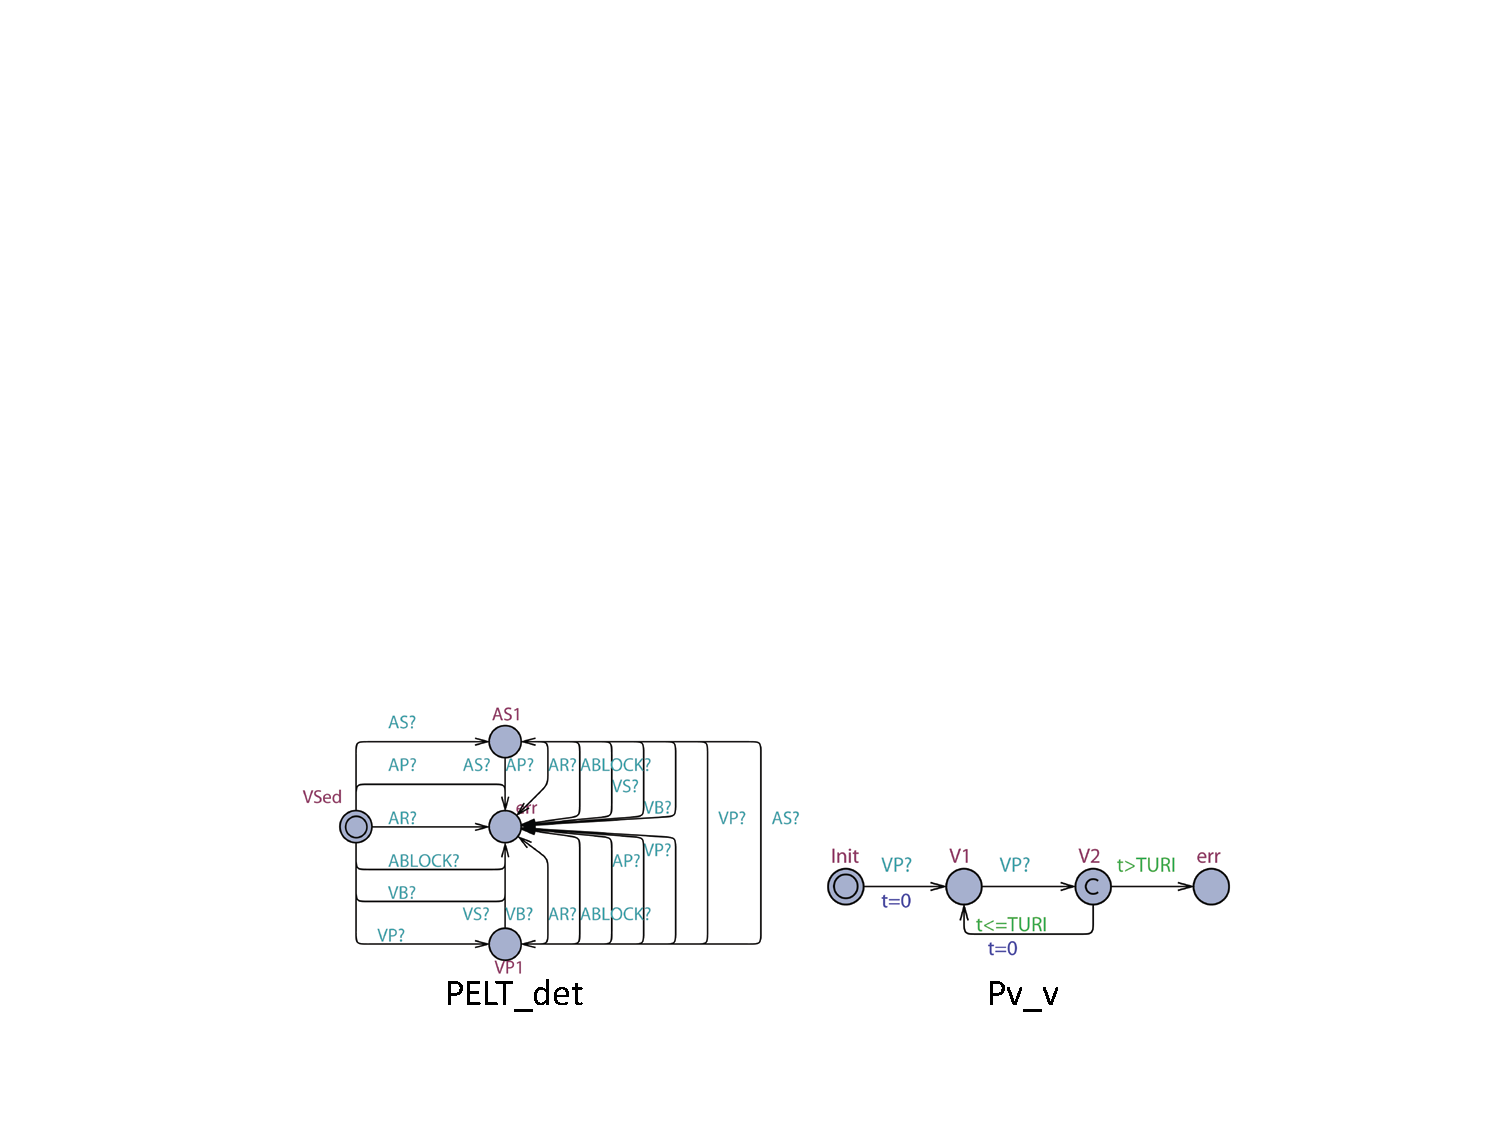
\includegraphics[width=0.7\textwidth]{figs/pelt_det.pdf}
		%%\vspace{-15pt}
		%\caption{\small (a) Any pattern other than VP-AS will result in error state (b) If the ventricular rate is slower than the Upper Rate Limit will go to error state}
		 %% \vspace{-15pt}
		%\label{fig:elt_det}
%\end{figure*}

Due to the limited information the pacemaker has about the heart, the pacemaker cannot distinguish a retrograde atrial event from an intrinsic atrial event which is triggered by the SA node. From the pacemaker's point of view, the pacemaker paces the ventricles as specified for every AS. That is why open-loop testing is unable to detect this closed-loop behavior. 

Modern pacemakers are equipped with anti-ELT algorithms to identify and terminate potential ELT. One common algorithm identifies ELT by the ELT pattern and terminates ELT by increasing TPVARP time once to block the AS caused by the V-A conduction. By increasing the blocking interval after a ventricular event, the pacemaker effectively ignores the early atrial signal detected due to the PVC.
\begin{figure*}
		\centering
		%\vspace{-10pt}
		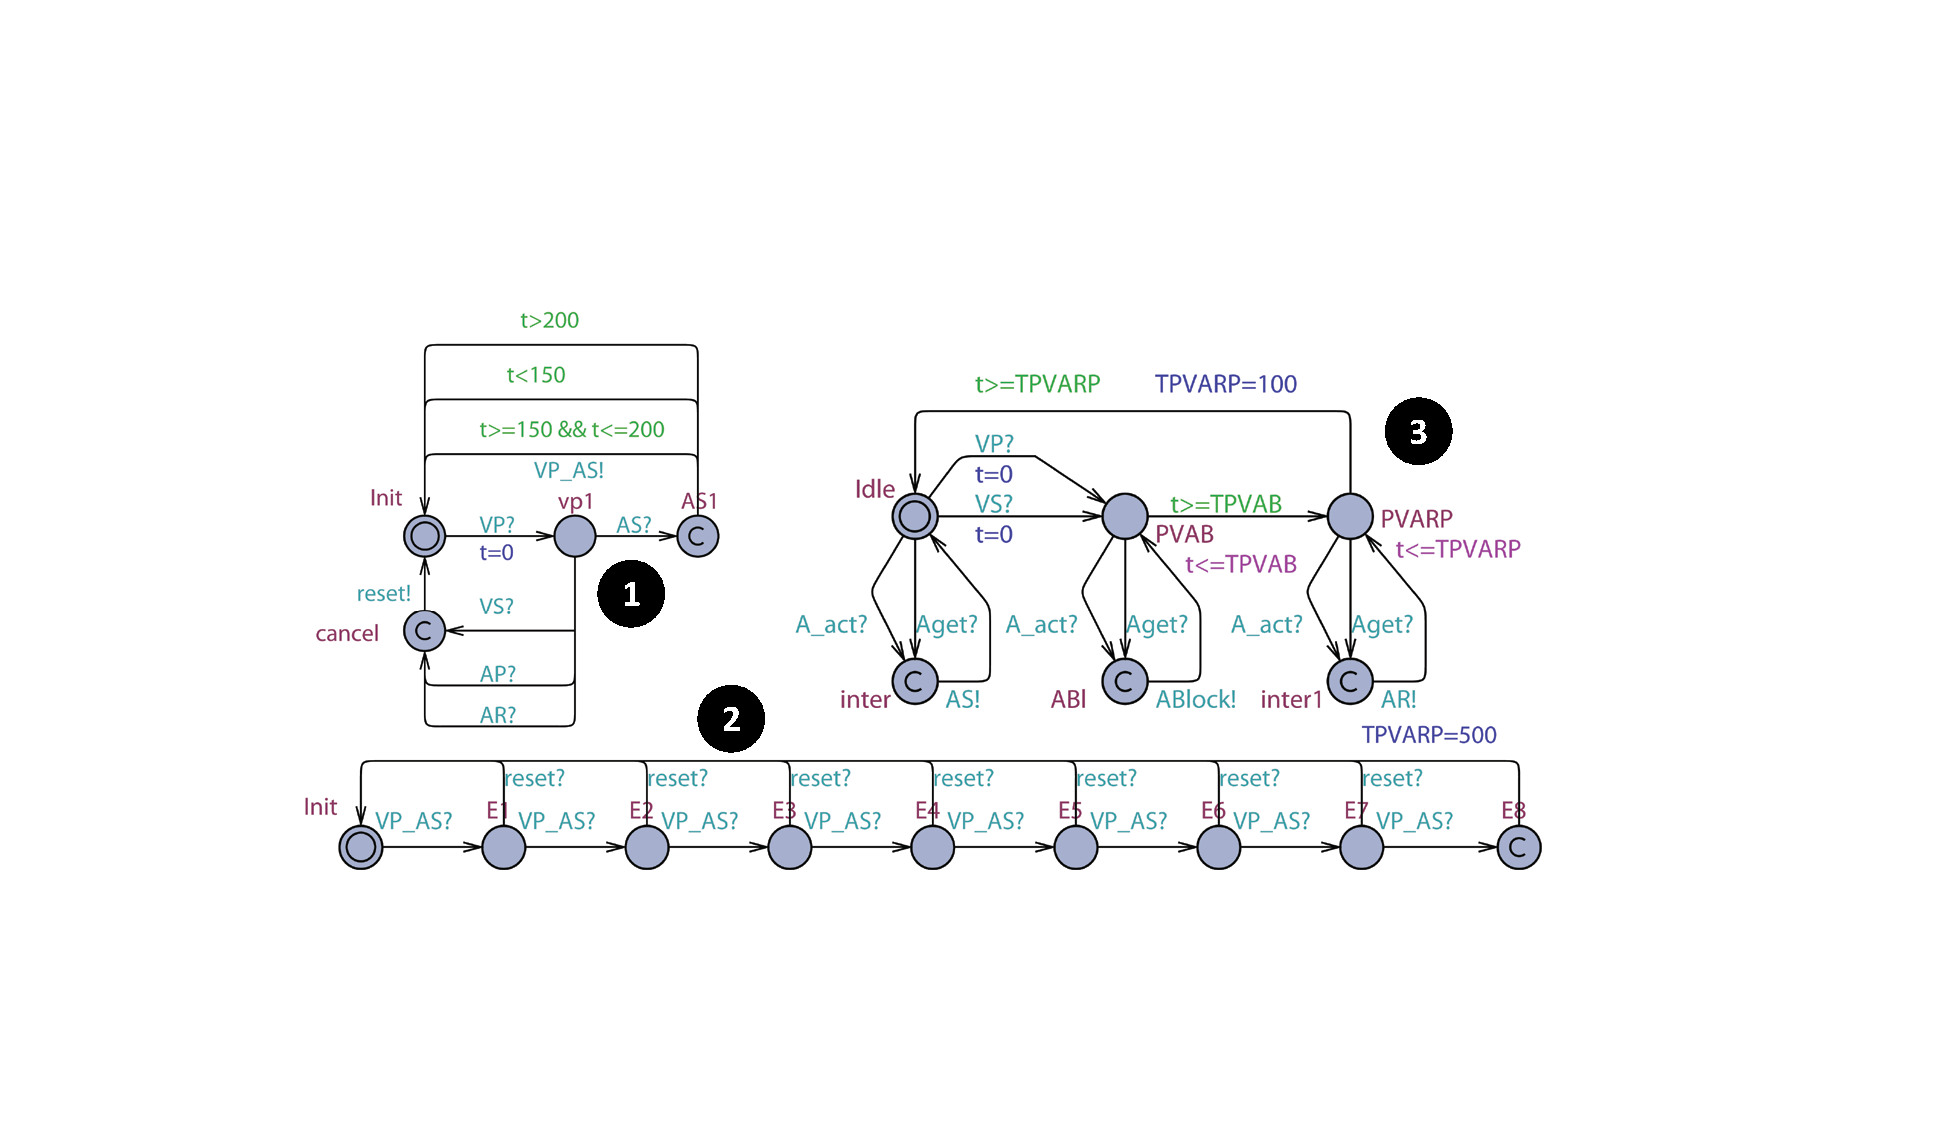
\includegraphics[width=0.7\textwidth]{figs/ELT_count.pdf}
		%\vspace{-20pt}
		\caption{\small (1) The component \textsf{PVAS} sends \textsf{VP\_AS!} event when a VP-AS pattern with delay between [150,200] is detected; (2) Component \textsf{ELTct}. After 8 VP-AS pattern, the algorithm increase TPVARP to 500ms. (3) Modified \textsf{PVARP'} component. TPVARP can only be set to 500 for one timing cycle.}
		 % \vspace{-15pt}
		\label{fig:ELT_count}
\end{figure*}
%\subsection{Existence of ELT}
%Two monitors were designed to show the existence of ELT. One monitor, \textsf{PELT\_det}, shows the persistence of the VP-AS pattern and the other monitor, \textsf{Pvv}, shows that the ventricular rate is always no slower than the upper rate limit (\figref{elt_det}). The property \\
%\textsf{$\varphi_{ELT}=$E[] ((not PELT\_det.err) $\&\&$ (not Pvv.err))}\\
%checks the existence of ELT behavior. After our initial verification we have:\\
%$H_4\|P\|PELT\_det\|Pvv\models\varphi_{ELT}$
%
%The evidence trace shows the behavior of the system. For simplicity we only show the state of the heart:\\
%$RE\|RE\xrightarrow[VP!\rightarrow Act\_node\_2!]{AVI.t\geq TAVI \wedge URI.t\geq TURI}$\\
%$RE\|RE\xrightarrow[Act\_path\_1!\rightarrow AS!]{N^1.t\geq 0}$\\
%$RE\|RE\xrightarrow[VP!\rightarrow Act\_node\_2!]{AVI.t\geq TAVI \wedge URI.t\geq TURI}$\\
%$RE\|RE\xrightarrow[Act\_path\_1!\rightarrow AS!]{N^1.t\geq 0}$\\
%$RE\|RE$
%
%\subsection{Trace Validation and Heart Model Refinement}
%We check this trace on more refined $H_3\| P$ and discovered that the trace above can correspond to two different scenarios:\\
%$RE\|AN\|RE\xrightarrow[VP!\rightarrow Act\_node\_2!]{AVI.t\geq TAVI \wedge URI.t\geq TURI}$\\
%$RE\|ID\|RE\xrightarrow[Act\_path\_1!\rightarrow AS!]{N^1.t\geq N^1.Trest\_min}$\\
%$RE\|AN\|RE\xrightarrow[VP!\rightarrow Act\_node\_2!]{AVI.t\geq TAVI \wedge URI.t\geq TURI}$\\
%$RE\|ID\|RE\xrightarrow[Act\_path\_1!\rightarrow AS!]{N^1.t\geq N^1.Trest\_min}$
%$RE\|AN\|RE$\\
%and\\
%$RE\|ID\|RE\xrightarrow[VP!\rightarrow Act\_node\_2!]{AVI.t\geq TAVI \wedge URI.t\geq TURI}$\\
%$RE\|RT\|RE\xrightarrow[Act\_node\_1!\rightarrow Act\_path\_1!\rightarrow AS!]{P.t\geq P.Tcond\_min}$\\
%$RE\|ID\|RE\xrightarrow[VP!\rightarrow Act\_node\_2!]{AVI.t\geq TAVI \wedge URI.t\geq TURI}$\\
%$RE\|RT\|RE\xrightarrow[Act\_node\_1!\rightarrow Act\_path\_1!\rightarrow AS!]{P.t\geq P.Tcond\_min}$\\
%$RE\|ID\|RE$
%
%Both traces correspond to actual clinical scenarios. However, the second trace corresponds to the ELT behavior which inappropriately increased the heart rate. By setting $N^1.Trest\_min\geq TURI$ in $H_3$ we can model the healthy heart and the first scenario will be eliminated. However, in $H_4$ the $Trest\_min$ is set to 0 so the two cases cannot be distinguished. So we use the refined heart model $H_3$ with $N^1.Trest\_min\geq TURI$.
%With the new heart model we have:\\
%$H_3\|P\|PELT\_det\|Pvv\models\varphi_{ELT}$\\
%The evidence trace, which is exactly the second trace above, shows exactly the ELT scenario.
%%\subsection{Heart Model Refinement 1}
%The property failed because the RHM cannot distinguish an intrinsic atrial event and a retrograde atrial event and we cannot set their parameters separately to represent a more complex heart condition. In order to deal with this problem, we refine our RHM by adding a non-deterministic A-V conduction \textsf{Cond\_n} (\figref{cond}) between the atrial channel and the ventricular channel. Events from \textsf{RHM\_A} can trigger ventricular event \textsf{V\_act!} with delay, which mimics the intrinsic A-V conduction. Ventricular events can trigger retrograde conduction to the atria, causing event \textsf{A\_retro!}. Since the intrinsic ventricular events are modeled by \textsf{Cond\_n}, \textsf{RHM\_V} is replaced with a PVC component (\figref{PXC}). The refined heart model \textsf{Refinement 1} is shown in \figref{refine}.
%\begin{figure}
%		\centering
%		%\vspace{-15pt}
%		\includegraphics[width=0.45\textwidth]{figs/cond.pdf}
%%		%\vspace{-20pt}
%		\caption{\small \textsf{Aget!} event can either trigger \textsf{V\_act!} event after delay or do nothing. \textsf{PVC!} event can either trigger \textsf{A\_retro!} event after delay or do nothing}
%		 %\vspace{-15pt}
%		\label{fig:cond}
%\end{figure}
%
%Since $\mathbb{T}(PVC)=\mathbb{R}$, we have $\mathbb{T}(PVC)\bigcup\mathbb{T}(V\_act)=\mathbb{R}$. We also have $\mathbb{T}(A\_retro)=\mathbb{T}(PVC)\bigcup\mathbb{T}(V\_act)$+ $[Tretromin, Tretromax]=\mathbb{R}$ and $\mathbb{T}(A\_retro)\bigcup\mathbb{T}(Aget)=\mathbb{R}$ thus the refinement is proper abstraction of the VHM. With the refined heart model we can adjust $\mathbb{T}(Aget)$ without changing $\mathbb{T}(A\_retro)$. The existence property holds and the evidence returned by UPPAAL shows an ELT execution trace.
%\begin{figure*}
%\centering
%%\vspace{-10pt}
		%\subfigure []{
				%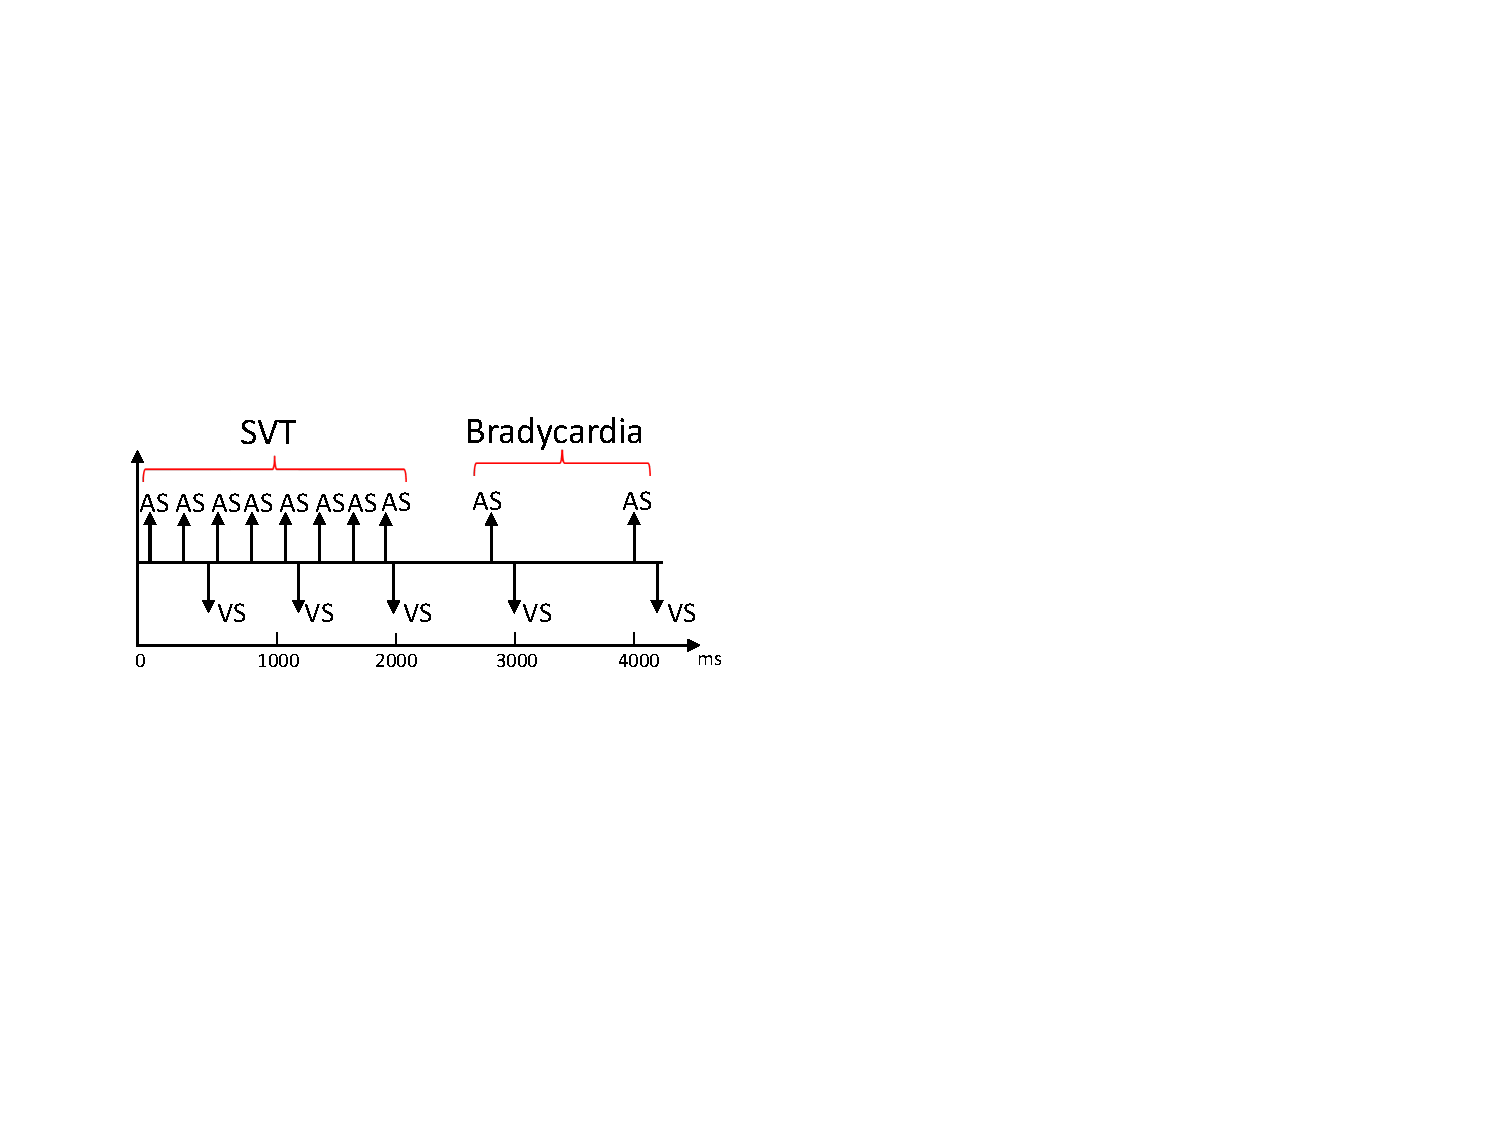
\includegraphics[width=0.4\textwidth]{figs/SVT_none.pdf}
				%\label{fig:SVT_none}
		%} 
		%\subfigure []{	
			%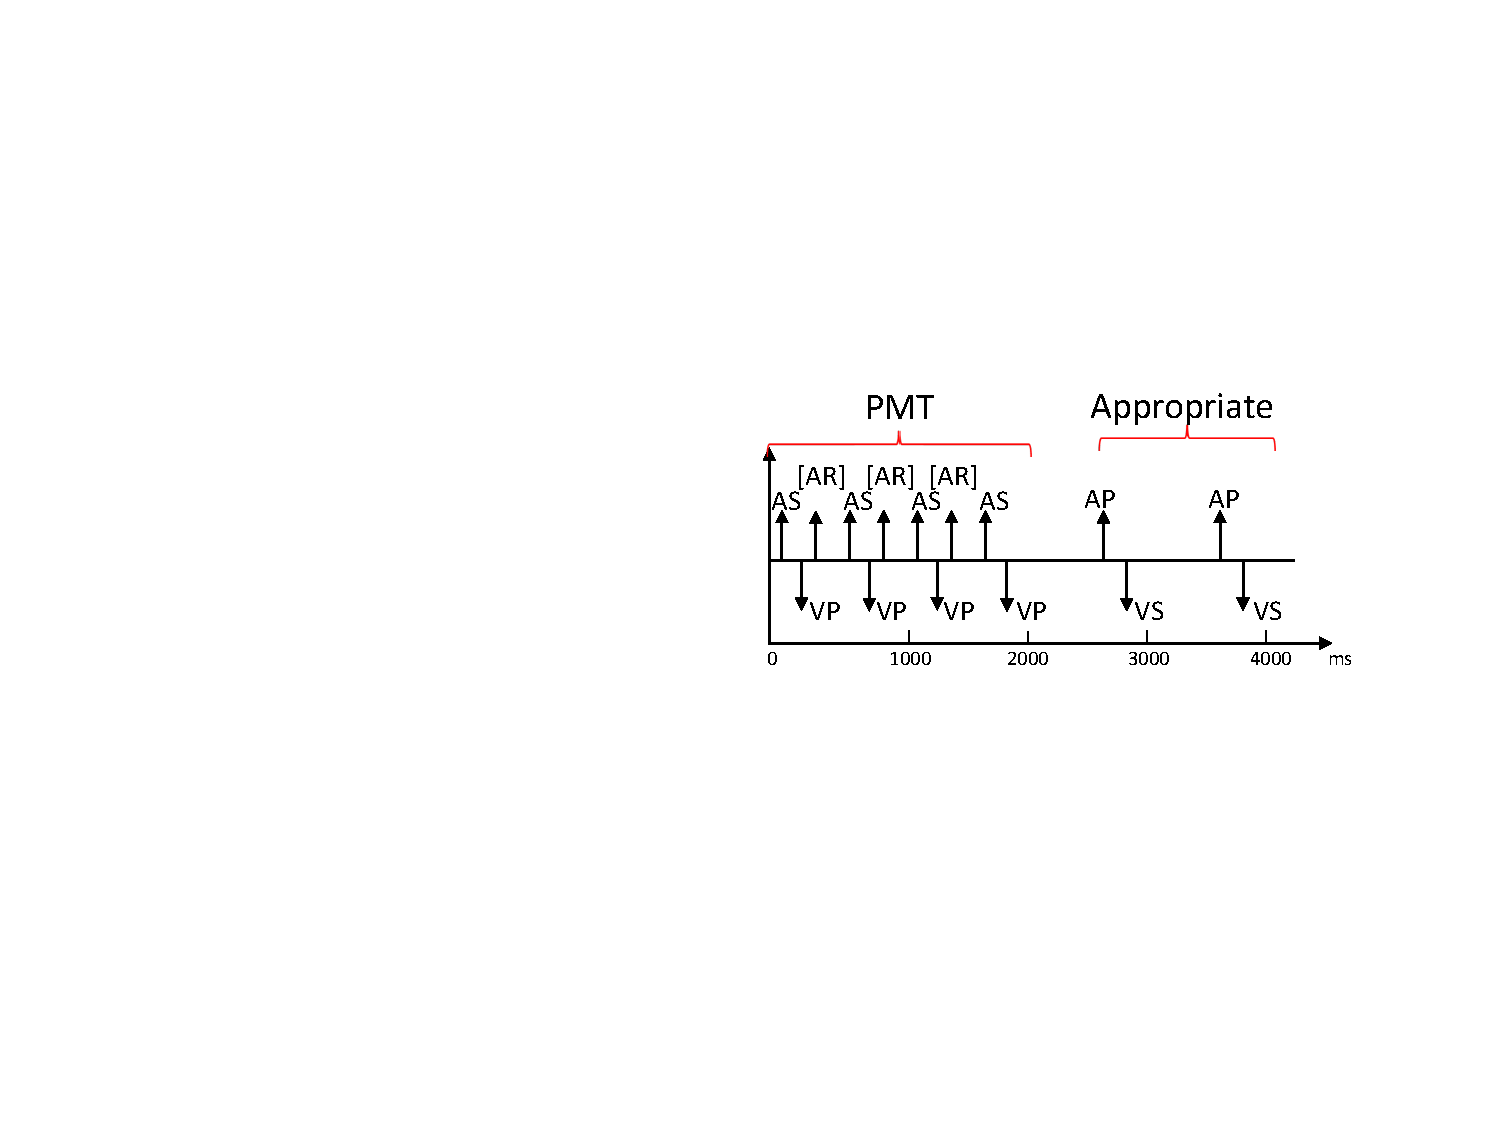
\includegraphics[width=0.4\textwidth]{figs/SVT_DDD.pdf}
			%\label{fig:SVT_DDD}
		%}
		%%\vspace{-10pt}
	%\caption{(a) Open-loop: 3:1 A-V conduction during SVT and low ventricular rate without SVT; (b) With DDD pacemaker: the pacemaker paces the ventricle for every atrial sense (AS), thus increase the ventricular rate inappropriately}
%\vspace{-10pt}
%\end{figure*} 
\subsubsection{ELT termination algorithm} 
The ELT persists without intervention and the patient's heart is forced to beat at a fast rate approaching the Upper Rate Limit. Thus, device manufacturers require a way to identify ELT and terminate it despite the limited information the pacemaker can get. The ELT detection algorithm by Boston Scientific \cite{challenge} utilizes these three features:
\begin{itemize}
  \item Ventricular rate at Upper Rate Limit
	\item VP-AS pattern
	\item Fixed V-A conduction delay
\end{itemize}
The pacemaker first monitors VP-AS pattern with ventricular rate at upper rate limit. Then it compares the VP-AS interval with previous intervals. ELT is confirmed if the difference between the current VP-AS interval and the first VP-AS interval is within $\pm$32ms for 8 consecutive times. Then the pacemaker increases the PVARP period to 500ms once so that the next AS will be blocked and will not trigger a VP, terminating ELT.
As the V-A conduction delays are patient-specific, the algorithm compares the VP-AS interval to a previously sensed value instead of an absolute value. Since we can not store past clock values in UPPAAL, we can not explicitly model this ELT detection algorithm. However, since the conduction delay in our heart model is within a known range, we can compare the VP-AS interval with this range. The VP-AS pattern detection module $VPAS$ for our anti-ELT algorithm is shown in \figref{ELT_count} (1). It detects the VP-AS pattern with ventricular rate at the Upper Rate Limit and sends out a \emph{VP\_AS} event if the interval qualifies. 

A counter $ELTct$ counts the number of qualified VP-AS patterns. It increases the PVARP period to 500ms if eight consecutive VP-AS patterns are detected. (\figref{ELT_count} (2)) The PVARP component is also modified so that the PVARP period can only be changed once by the anti-ELT algorithm. (\figref{ELT_count} (3))

\subsubsection{Verification of the algorithm}
With the new pacemaker model\\ 
$P_1=LRI\|AVI\|URI\|PVARP'\|VRP\|ELTct\|VPAS$\\
we first check whether the two efficacy properties still hold when the anti-ELT algorithm is introduced. We have 
$$H_0\|P_1\|PLRI\_test\models\varphi_{LRI}$$
$$H_0\|P_1\|PURI\_test\models\varphi_{URI}$$
Indicating the efficacy properties still hold after introducing the anti-ELT algorithm.

Then property $\varphi_{PMT}$ is checked, we have
$$H2\_4\|P_1\|PELT\_det\|Pvv\not\models\varphi_{PMT}$$
which indicates the algorithm successfully eliminated all ELT executions.

\subsection{Mode Switch Operation: Atrial Tachycardia Response}
\label{Mode_switch}

Pacemaker manufacturers have designed algorithms to detect and terminate behaviors as in $CE_{af}$. Intuitively, the mode-switch algorithm first detects SVT. After confirmed detection, it switches the pacemaker from a dual-chamber mode to a single-chamber mode. During the single-chamber mode, the A-V synchrony function of the pacemaker is deactivated thus the ventricular rate is decoupled from the fast atrial rate. After the algorithm determines the end of SVT, it will switch the pacemaker back to the dual chamber mode. 
\begin{figure*}
		\centering
		%\vspace{-19pt}
		\includegraphics[width=0.8\textwidth]{figs/AVI_ms.pdf}
		%\vspace{-10pt}
		\caption{\small (a) After switching to \textsf{VDI} mode, the new LRI component \textsf{LRI'} maintains a minimum V-V interval; (b) After switching to \textsf{VDI} mode, the new AVI component \textsf{AVI'} keeps track of the time after each atrial events.}
		%  \vspace{-20pt}
		\label{fig:avi_ms}
\end{figure*}
The mode-switch algorithm (also known as atrial tachycardia response) specification we use is similar to the one described in the Boston Scientific pacemakers' manual (\cite{compass}). The algorithm first measures the interval between atrial events outside the blanking period (AS, AR). The interval is considered as \emph{fast} if it is above a threshold (\emph{Trigger Rate}) and \emph{slow} otherwise. In our UPPAAL model we model it as $INT$ (see \figref{dur_count} (1)). A counter $CNT$ increments for \emph{fast} events and decrements for \emph{slow} events (see \figref{dur_count} (2)). After the counter value reaches the \emph{Entry Count}, the algorithm will start a \emph{Duration} ($DUR$) ,which is a time interval used to confirm the detection of SVT (see \figref{dur_count} (3)). In the \emph{Duration}, the counter keeps counting. If the counter value is still positive after the \emph{Duration}, the pacemaker will switch to the VDI mode (\emph{Fallback mode}). In the VDI mode, the pacemaker only senses and paces the ventricle. At any time if the counter reaches zero, the \emph{Duration} will terminate and the pacemaker is switched back to DDD mode.
% to show some interesting findings. The basic idea of this simplified model is explained in detail. \\
%\mySubSubSection{UPPAAL model for mode-switch algorithm}
In our UPPAAL model of the mode-switch algorithm, we use nominal parameter values from the clinical setting. We define \emph{trigger rate} at 170bpm (350ms), \emph{entry count} at 8, \emph{duration} for 8 ventricular events and \emph{fallback mode} as VDI. 
\begin{figure*}
		\centering
				%\vspace{-15pt}
		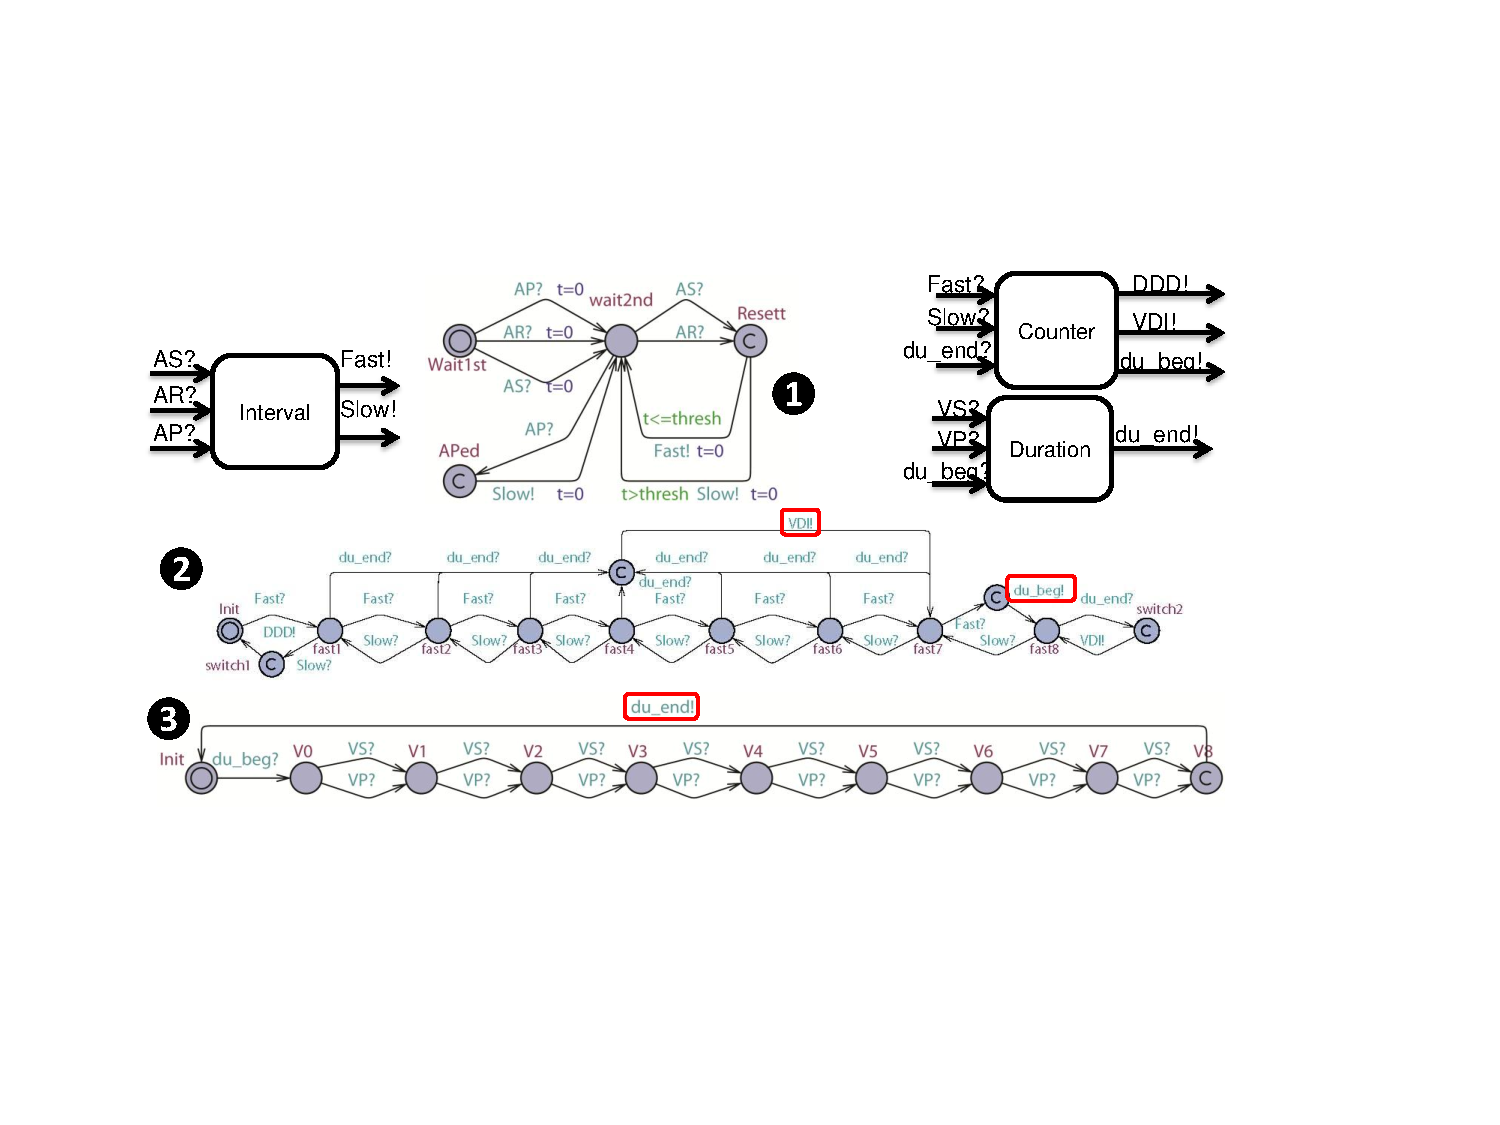
\includegraphics[width=0.9\textwidth]{figs/duration.pdf}
		%\vspace{-10pt}
		\caption{\small (1) Component \textsf{INT}: An atrial event (\textsf{AS,AR}) arrives before \textsf{thresh} after the previous atrial event is regarded as a \textsf{fast} event. Atrial event arrives after \textsf{thresh} and \textsf{AP} are regarded as \textsf{slow} event; (2) Component \textsf{CNT}: After 8 \textsf{fast} event the algorithm will start a duration by sending \textsf{du\_beg} and will switch to \textsf{VDI} mode when the duration ends (\textsf{du\_end}); (3) Component \textsf{DUR} :The duration length is 8 ventricular events (\textsf{VS,VP})}
		  %\vspace{-15pt}
		\label{fig:dur_count}
\end{figure*} 

In order to model both DDD and VDI modes and the switching between them, we made modifications to the AVI and LRI components.
In each component two copies for both modes are modeled, and switch between each other when switching events (DDD, VDI) are received. During VDI mode, \textsf{VP} is delivered by the LRI component instead of the AVI component. The clock values are shared between both copies in order to preserve essential intervals even after switching. The modified AVI ($AVI'$) and LRI ($LRI'$)components are shown in \figref{avi_ms}. 

\subsubsection{Verification of the Mode-Switch Algorithm}
With the new pacemaker model\\ 
$P_2=LRI'\|AVI'\|URI\|PVARP'\|VRP\|INT\|CNT\|DUR$\\
we first check whether the two efficacy properties still hold when the anti-ELT algorithm is introduced. We have 
$$H_0\|P_2\|PLRI\_test\not\models\varphi_{LRI}$$
$$H_0\|P_2\|PURI\_test\models\varphi_{URI}$$
By analyzing the counter-example we found that when the pacemaker is switching from VDI mode to DDD mode, the responsibility to deliver VP switched from LRI component to AVI component. Since the clock reference is different (Ventricular events in LRI component and Atrial events in AVI component), the clock value for delivering the next VP is not preserved. As a result, if an atrial event which triggered the mode-switch from VDI to DDD happens within [TLRI-TAVI, TLRI) after the last ventricular event, the next ventricular pacing will be delayed by at most TAVI time, which violates the Lower Rate Limit property (\figref{safety}). 
%%\begin{figure}
%%		\centering
%%		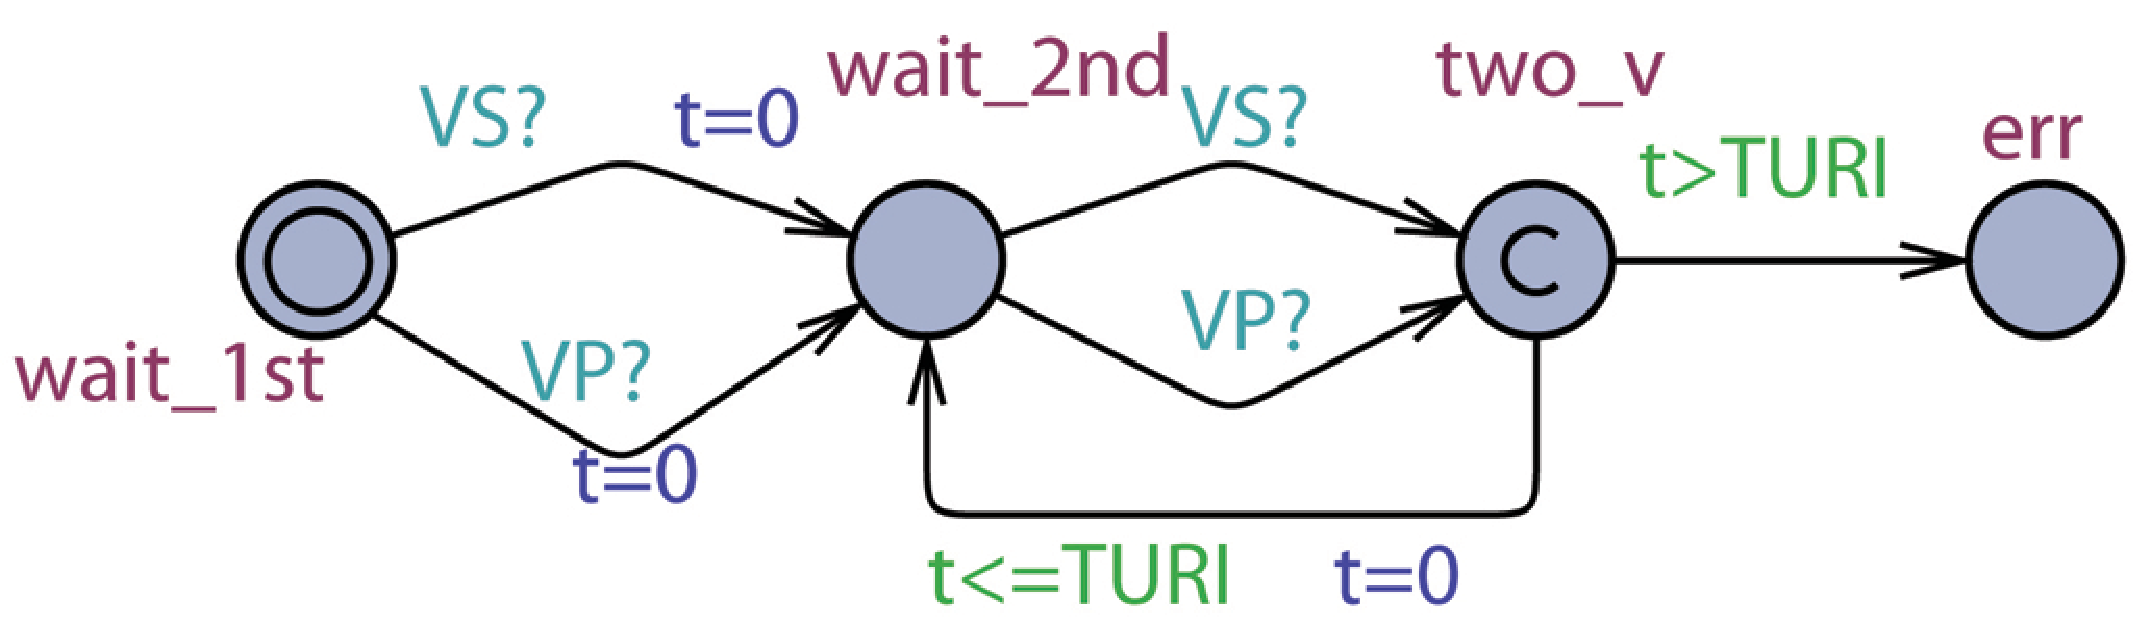
\includegraphics[width=0.4\textwidth]{figs/vv.pdf}
%%		\caption{\small Monitor \textsf{Pv\_v} for SVT: There exists an endless sequence in which interval between ventricular events is at most TURI}
%%		  %\vspace{-15pt}
%%		\label{fig:vv}
%%\end{figure}
Then property $\varphi_{PMT}$ is checked, we have
$$H3\_2\|P_1\|PELT\_det\|Pvv\not\models\varphi_{PMT}$$
Indicating the mode-switch algorithm failed to eliminate the PMT scenario. The counter-example trace returned by UPPAAL shows that a subset of atrial events fall into the blanking period after a ventricular event (see \figref{liveness}). As a result, two fast events are reduced to one slow event and mode switch may never happen. Therefore the mode-switch algorithm in our pacemaker model can not terminate all PMT behaviors as specified as certain mild PMT events are admissible.
\begin{figure}
\centering
%\vspace{-20pt}
		\subfigure []{
				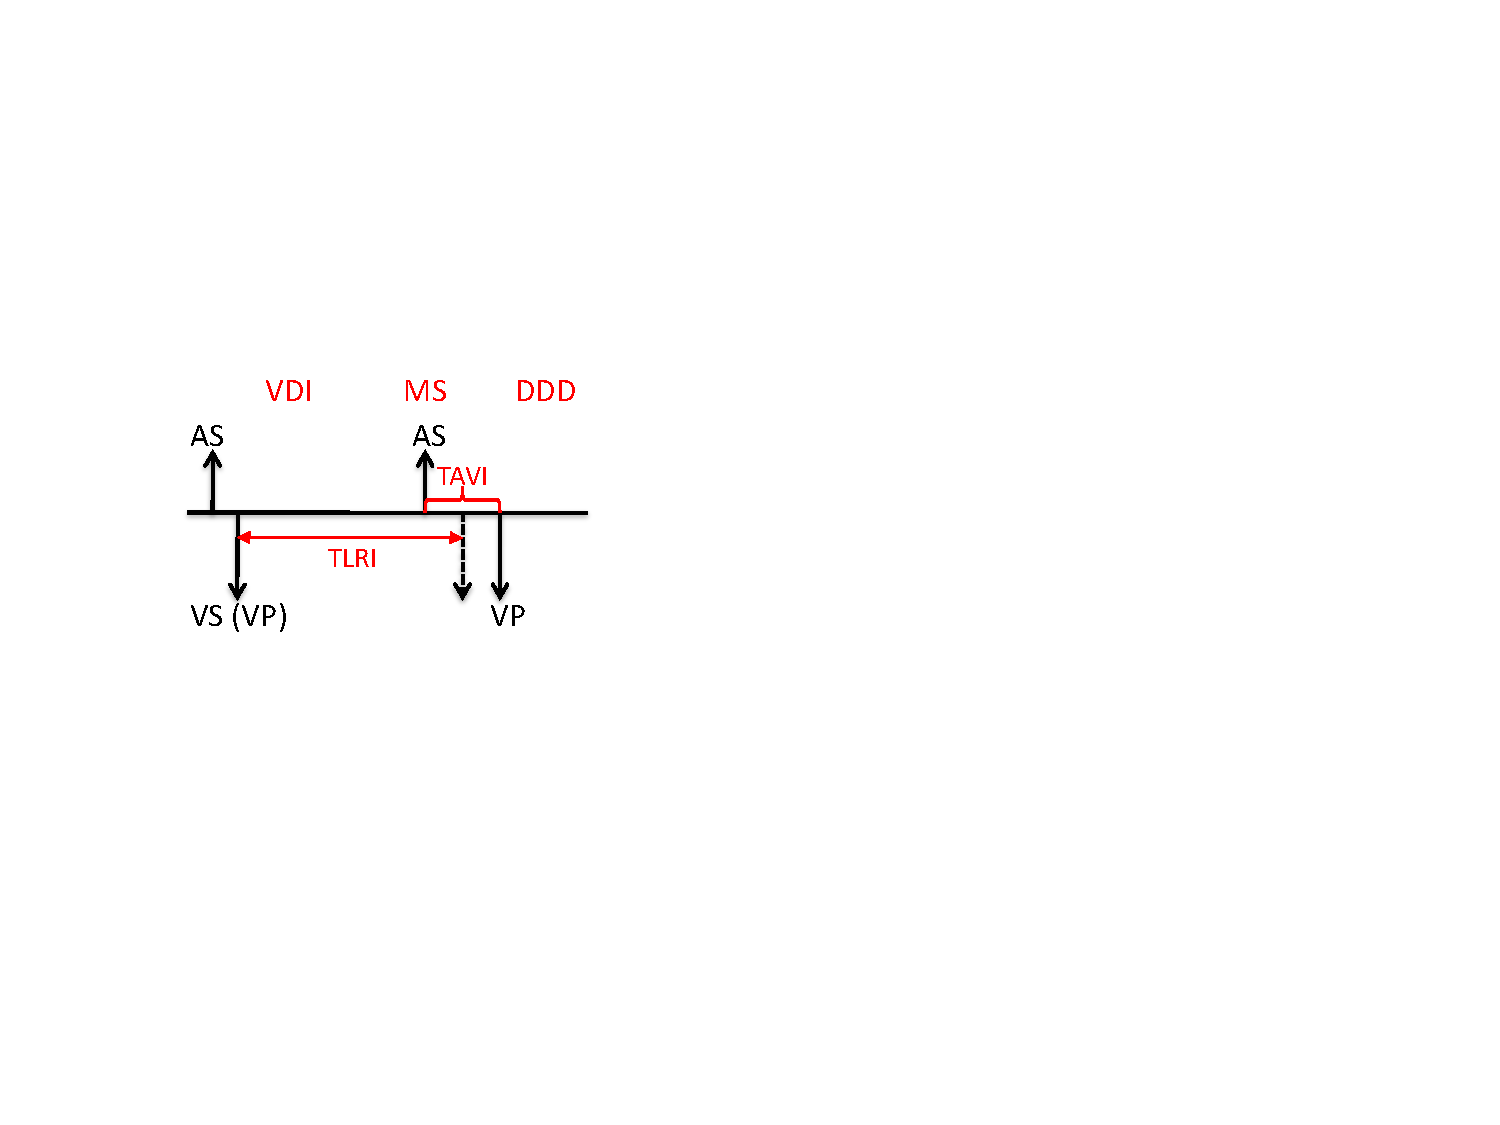
\includegraphics[width=0.4\textwidth]{figs/safety.pdf}
				\label{fig:safety}
		} 
		\subfigure []{	
			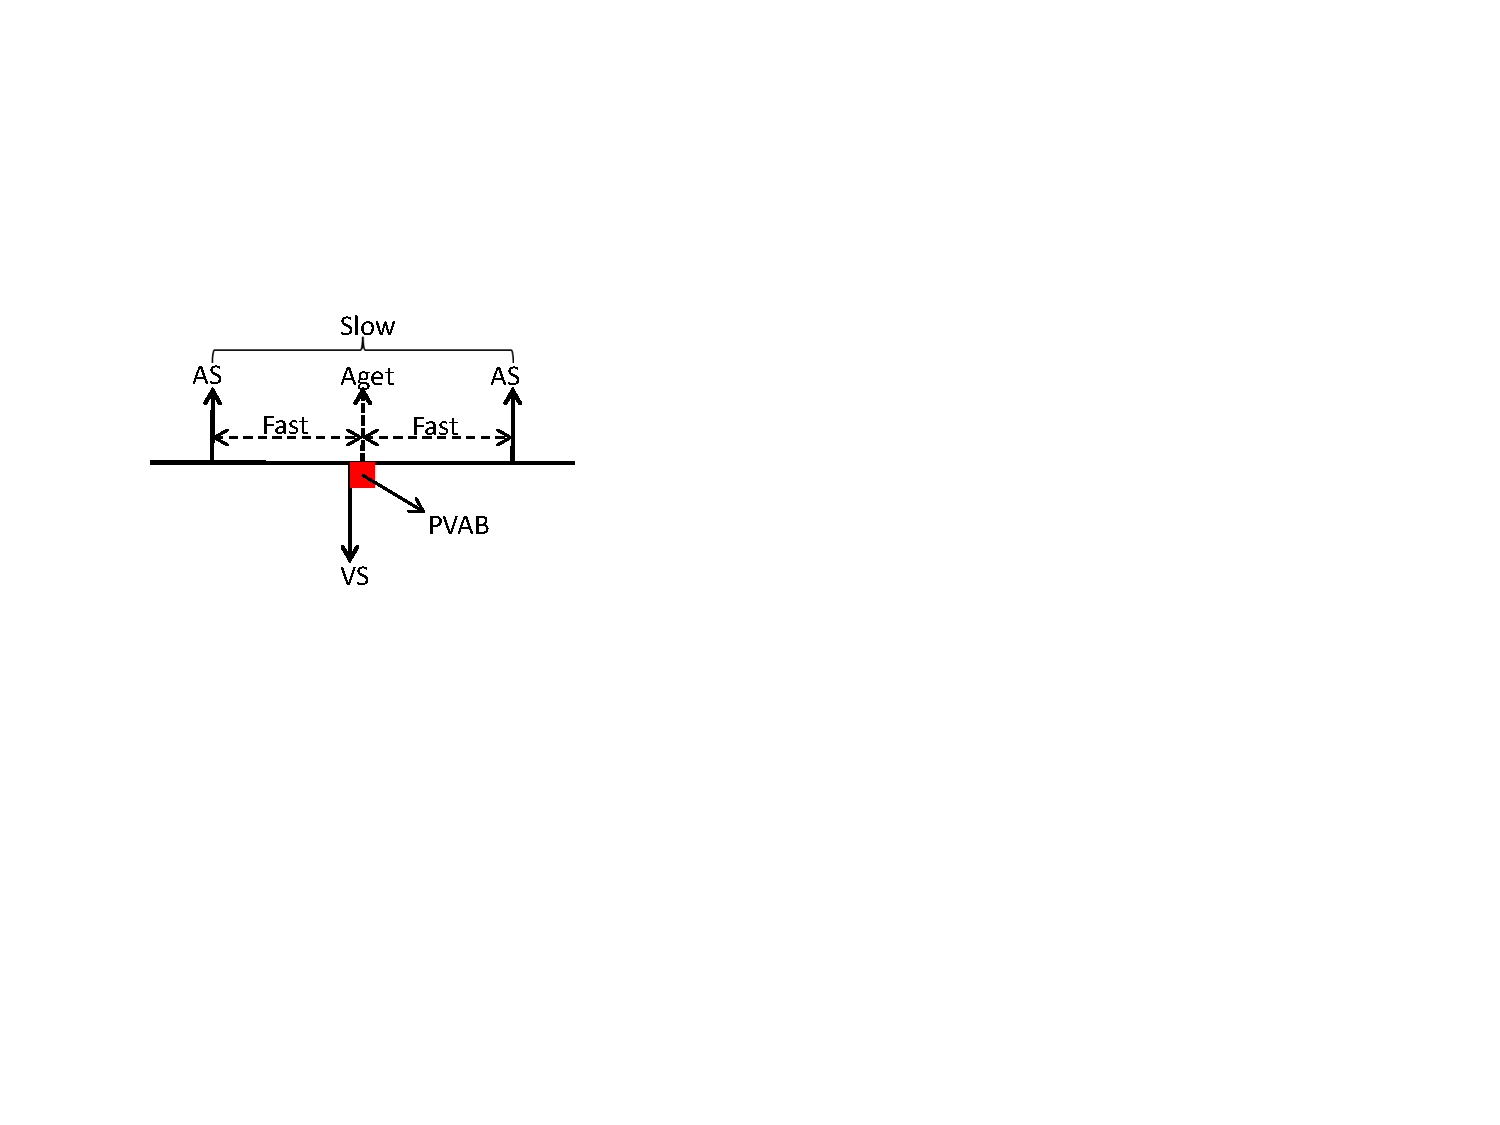
\includegraphics[width=0.4\textwidth]{figs/liveness.pdf}
			\label{fig:liveness}
		}
	\caption{(a) Safety Violation: VP is delayed due to the reset of timer during mode-switch, (b) Efficacy Violation: The blocking period may block some atrial events, turning two \emph{Fast} events to one \emph{Slow} event (\cite{TACAS12}})
\end{figure} 

\section{Discussion}
Model checking is not widely use in industry, in part, due to scalability issues and also because domain expertise must be a skill possessed by the verification engineer. 
However, with rigorous abstraction of the system and its environment, model checking can be used to identify 
known and even unknown mechanisms to induce hazards. 
In this chapter, we used a model of a dual chamber pacemaker as an example to demonstrate the use of model checking during risk analysis. 
During the process we identified the need to refine the heart models to eliminate false-positives introduced during the abstraction, and demonstrated the difficulty to do so manually. 
The abstraction tree approach is then proposed to reduce the effort needed for both the developers and the domain experts, which makes model checking a viable approach for providing safety and effectiveness evidence. 
With the abstraction tree of heart models, safety and efficacy violations are identified within the pacemaker specification, which demonstrates the capability of model checking to identify issues during the early development of autonomous medical devices.
